%% Submissions for peer-review must enable line-numbering 
%% using the lineno option in the \documentclass command.
%%
%% Preprints and camera-ready submissions do not need 
%% line numbers, and should have this option removed.
%%
%% Please note that the line numbering option requires
%% version 1.1 or newer of the wlpeerj.cls file, and
%% the corresponding author info requires v1.2

\documentclass[fleqn,10pt,lineno]{wlpeerj} % for journal submissions
%\documentclass[fleqn,10pt]{wlpeerj} % for preprint submissions

%\newcommand{\rr}{${\mathcal{R}}$}
\usepackage{bbding} %for FiveStarOpen
\usepackage{changepage} % for adjustwidth
\usepackage{amssymb}
\usepackage{amsmath}
\usepackage{upgreek}
\usepackage[]{fontenc}
\usepackage{color}
\usepackage{bm}
\usepackage[english]{babel}
\usepackage{graphicx}
\usepackage{tikz}
\usetikzlibrary{positioning}
\usepackage{ifthen}
\usepackage{xstring}
\usepackage{afterpage}
%\usepackage[hidelinks]{hyperref}
\usepackage[colorlinks=true, allcolors=blue, pdfborder={0 0 0}]{hyperref}

\newcommand{\floor}[1]{\left \lfloor #1 \right \rfloor}
\newcommand{\round}[1]{\left \lfloor #1 \right \rceil }
\newcommand{\ceil}[1]{\left \lceil #1 \right \rceil }
\newcommand{\Fig}[1]{Fig.~\ref{#1}}
%\newcommand{\Fig}[1]{Figure~\ref{#1}}
\newcommand{\Figs}[1]{Figs.~\ref{#1}}
%\newcommand{\Figs}[1]{Figures~\ref{#1}}
\newcommand{\Sec}[1]{Section~\ref{#1}}
\newcommand{\Secs}[1]{Sections~\ref{#1}}
\newcommand{\Chap}[1]{Chapter~\ref{#1}}
\newcommand{\Chaps}[1]{Chapters~\ref{#1}}
\newcommand{\Tab}[1]{Table~\ref{#1}}
\newcommand{\Tabs}[1]{Tables~\ref{#1}}
\newcommand{\Eqn}[1]{Eqn.~\ref{#1}}
\newcommand{\Eqns}[1]{Eqns.~\ref{#1}}
\newcommand{\InEqn}[1]{Inequality~(\ref{#1})}
\newcommand{\InEqns}[1]{Inequalities~(\ref{#1})}
\newcommand{\Center}[1]{\textcolor{white}{.}\hfill#1\hfill\textcolor{white}{.}}
\newcommand{\ang}{$\textrm\AA$\xspace}
\newcommand{\new}[1]{#1}
\newcommand{\New}[1]{#1}
\newcommand{\n}[1]{#1}
\newcommand{\we}{I~}

\newcommand\solidrule[1][1cm]{\rule[0.5ex]{#1}{0.2mm}}
\newcommand\dotdashedrule{\mbox{%
  \solidrule[1.5mm]\hspace{0.75mm}\solidrule[0.2mm]\hspace{0.75mm}\solidrule[1.5mm]}}
\newcommand\dashedrule{\mbox{%
  \solidrule[1.5mm]\hspace{0.75mm}\solidrule[1.5mm]}}
\newcommand\dottedrule{\mbox{%
  \solidrule[0.2mm]\hspace{0.3mm}\solidrule[0.2mm]\hspace{0.3mm}\solidrule[0.2mm]\hspace{0.3mm}\solidrule[0.2mm]\hspace{0.3mm}\solidrule[0.2mm]\hspace{0.3mm}\solidrule[0.2mm]}}
  
  
\usepackage{xspace}

\newcommand{\pname}{\texttt{plotMAP}\xspace}
\newcommand{\code}[1]{\texttt{#1}\xspace}

\usepackage[cal=cm,scrscaled=1.05]{mathalfa} % This is for \mathcal{}, particularly \mathcal{R}
\DeclareMathAlphabet\mathbfcal{OMS}{cmsy}{b}{n} % for boldface mathcal: \mathbfcal{}
\newcommand{\rr}{$\mathcal{R}$\xspace}


\def\kt{k_{\rm B}T}


\def\beq{\begin{equation}}
\def\eeq{\end{equation}}
\def\bea{\begin{eqnarray}}
\def\eea{\end{eqnarray}}

\def\cal#1{\mathcal{#1}}
\def\eqq#1{Eq.~(\ref{#1})}
\def\eq#1{(\ref{#1})}
\def\av#1{\langle #1 \rangle}

\def\f#1{Fig.~\ref{#1}}
\def\ff#1{Figs.~\ref{#1}}

\def\s#1{Section~\ref{#1}}

\def\c#1{~\cite{#1}}


%\newcommand{\c}[1]{\citep{#1}}

\newcommand{\figdir}{./figures}

\title{On the other hand: chirality and the peptide backbone}

\author[1,*]{Ranjan V. Mannige}
%\author[1]{Other Names TBD}
\affil[1]{~Molecular Foundry, Lawrence Berkeley National Laboratory, Berkeley, CA, U.S.A.}
\affil[*]{~rvmannige@lbl.gov}

% \keywords{Protein structure, Backbone Chirality, Backbone Twist}

\begin{abstract}
Proteins and peptides comprise a class of biomolecules that display diverse conformations, which is the reason for their diverse functionality. These conformations are afforded in large part due to a protein's backbone, whose twists and contortions allow for a protein to fold into particular conformations. The Ramachandran plot describes a backbone as a function of its dominant degrees of freedom -- the backbone dihedral angles $\phi$ and $\psi$ \citep{Ramachandran1963}. Since its introduction in the 1960s, Ramachandran plots have been a crucial tool to characterize protein backbone features. 
However, so far, the exact nature of the twist of a backbone, as a function of $\phi$ and $\psi$ has not been completely described for both $cis$ and $trans$ backbones. 
In these lines, this short paper provides 1) a simple metric ($\chi$) for backbone chirality, 2) rules of thumb as to how to interpret chirality within a Ramachandran plot, and 3) a complete characterization of the way a backbone twists in all regions of the Ramachandran plot for both $cis$ and $trans$ backbones; this fills in the `dead space' within the Ramachandran plot, which are regions that are not commonly accessed by proteins. Given the recent discussion on intrinsic disorder, whose locations on the Ramachandran plot are not well characterized, and new peptide mimics that are not bound by traditional peptide rules, these results aim to serve as a guide for understanding new types of peptide and peptidomimetic structures. Finally, we provide Python scripts that replicate the results within the paper as a GitHub repository.
\end{abstract}

\begin{document}

\flushbottom
\maketitle
\thispagestyle{empty}

\section*{Introduction}

Proteins and peptides are a class of biomolecules that are unparalleled in their functionality \citep{Berg2006}. 
They are able to display diverse functions because of the diverse conformations that they display. 
When attempting to characterize a protein's conformation, it is useful to recognize that proteins are linear polymers:  beads on a chain, where beads are amino acids, otherwise called residues (\Fig{fig:intro}a). These polymers may be distinguished into two regions: the backbone (dark bonds in \Fig{fig:intro}a) and residue-specific sidechains that `decorate' the backbone (the `R's in \Fig{fig:intro}a). Therefore, a protein's conformation is highly dependent on the manner in which a backbone curves in space. For any protein, its collection or ensemble of conformations\footnote{These conformations can be specific folds in globular proteins or larger structural ensembles in intrinsically disordered proteins; \cite{Mannige2014b}.} define possible molecular functionality. 
In short, understanding how a backbone behaves is of great importance to the field of biochemistry, since understanding the structure of a protein goes a long way towards understanding how proteins function. 

\cite{Ramachandran1963} recognized that the twist of a protein or peptide backbone is dependent on the dihedral angles $\phi$ and $\psi$ (\Fig{fig:intro}a)\footnote{Another degree of freedom -- the amide dihedral angle ($\omega$) -- that is predominantly $trans$ in peptides (i.e., $\omega = 180^\circ$), but which can also occupy $cis$ conformations ($\omega = 0^\circ$). The Ramachandran plot requires a presumption that the backbone is either $cis$ or $trans$.}. 
Any peptide built with uniform twist or backbone parameters (say, $\phi=X^\circ$ and $\psi=Y^\circ$) will result in a regular structure; some regular structures are energetically stable (or metastable) and are called secondary structures (\Fig{fig:intro}b). These secondary structures pack together with the help of loops, which are also twisted \citep{Berg2006}. Today, two-dimensional $(\phi,\psi)$ plots are called Ramachandran plots, and have been used as a guide for understanding a peptide backbone's general conformational state or `twistedness' at a glance \citep{Ho2003,Berg2006,Alberts2002,Subramanian2001,Laskowski1993,Hooft1997,Laskowski2003}.

\begin{figure}[t!]
\centering
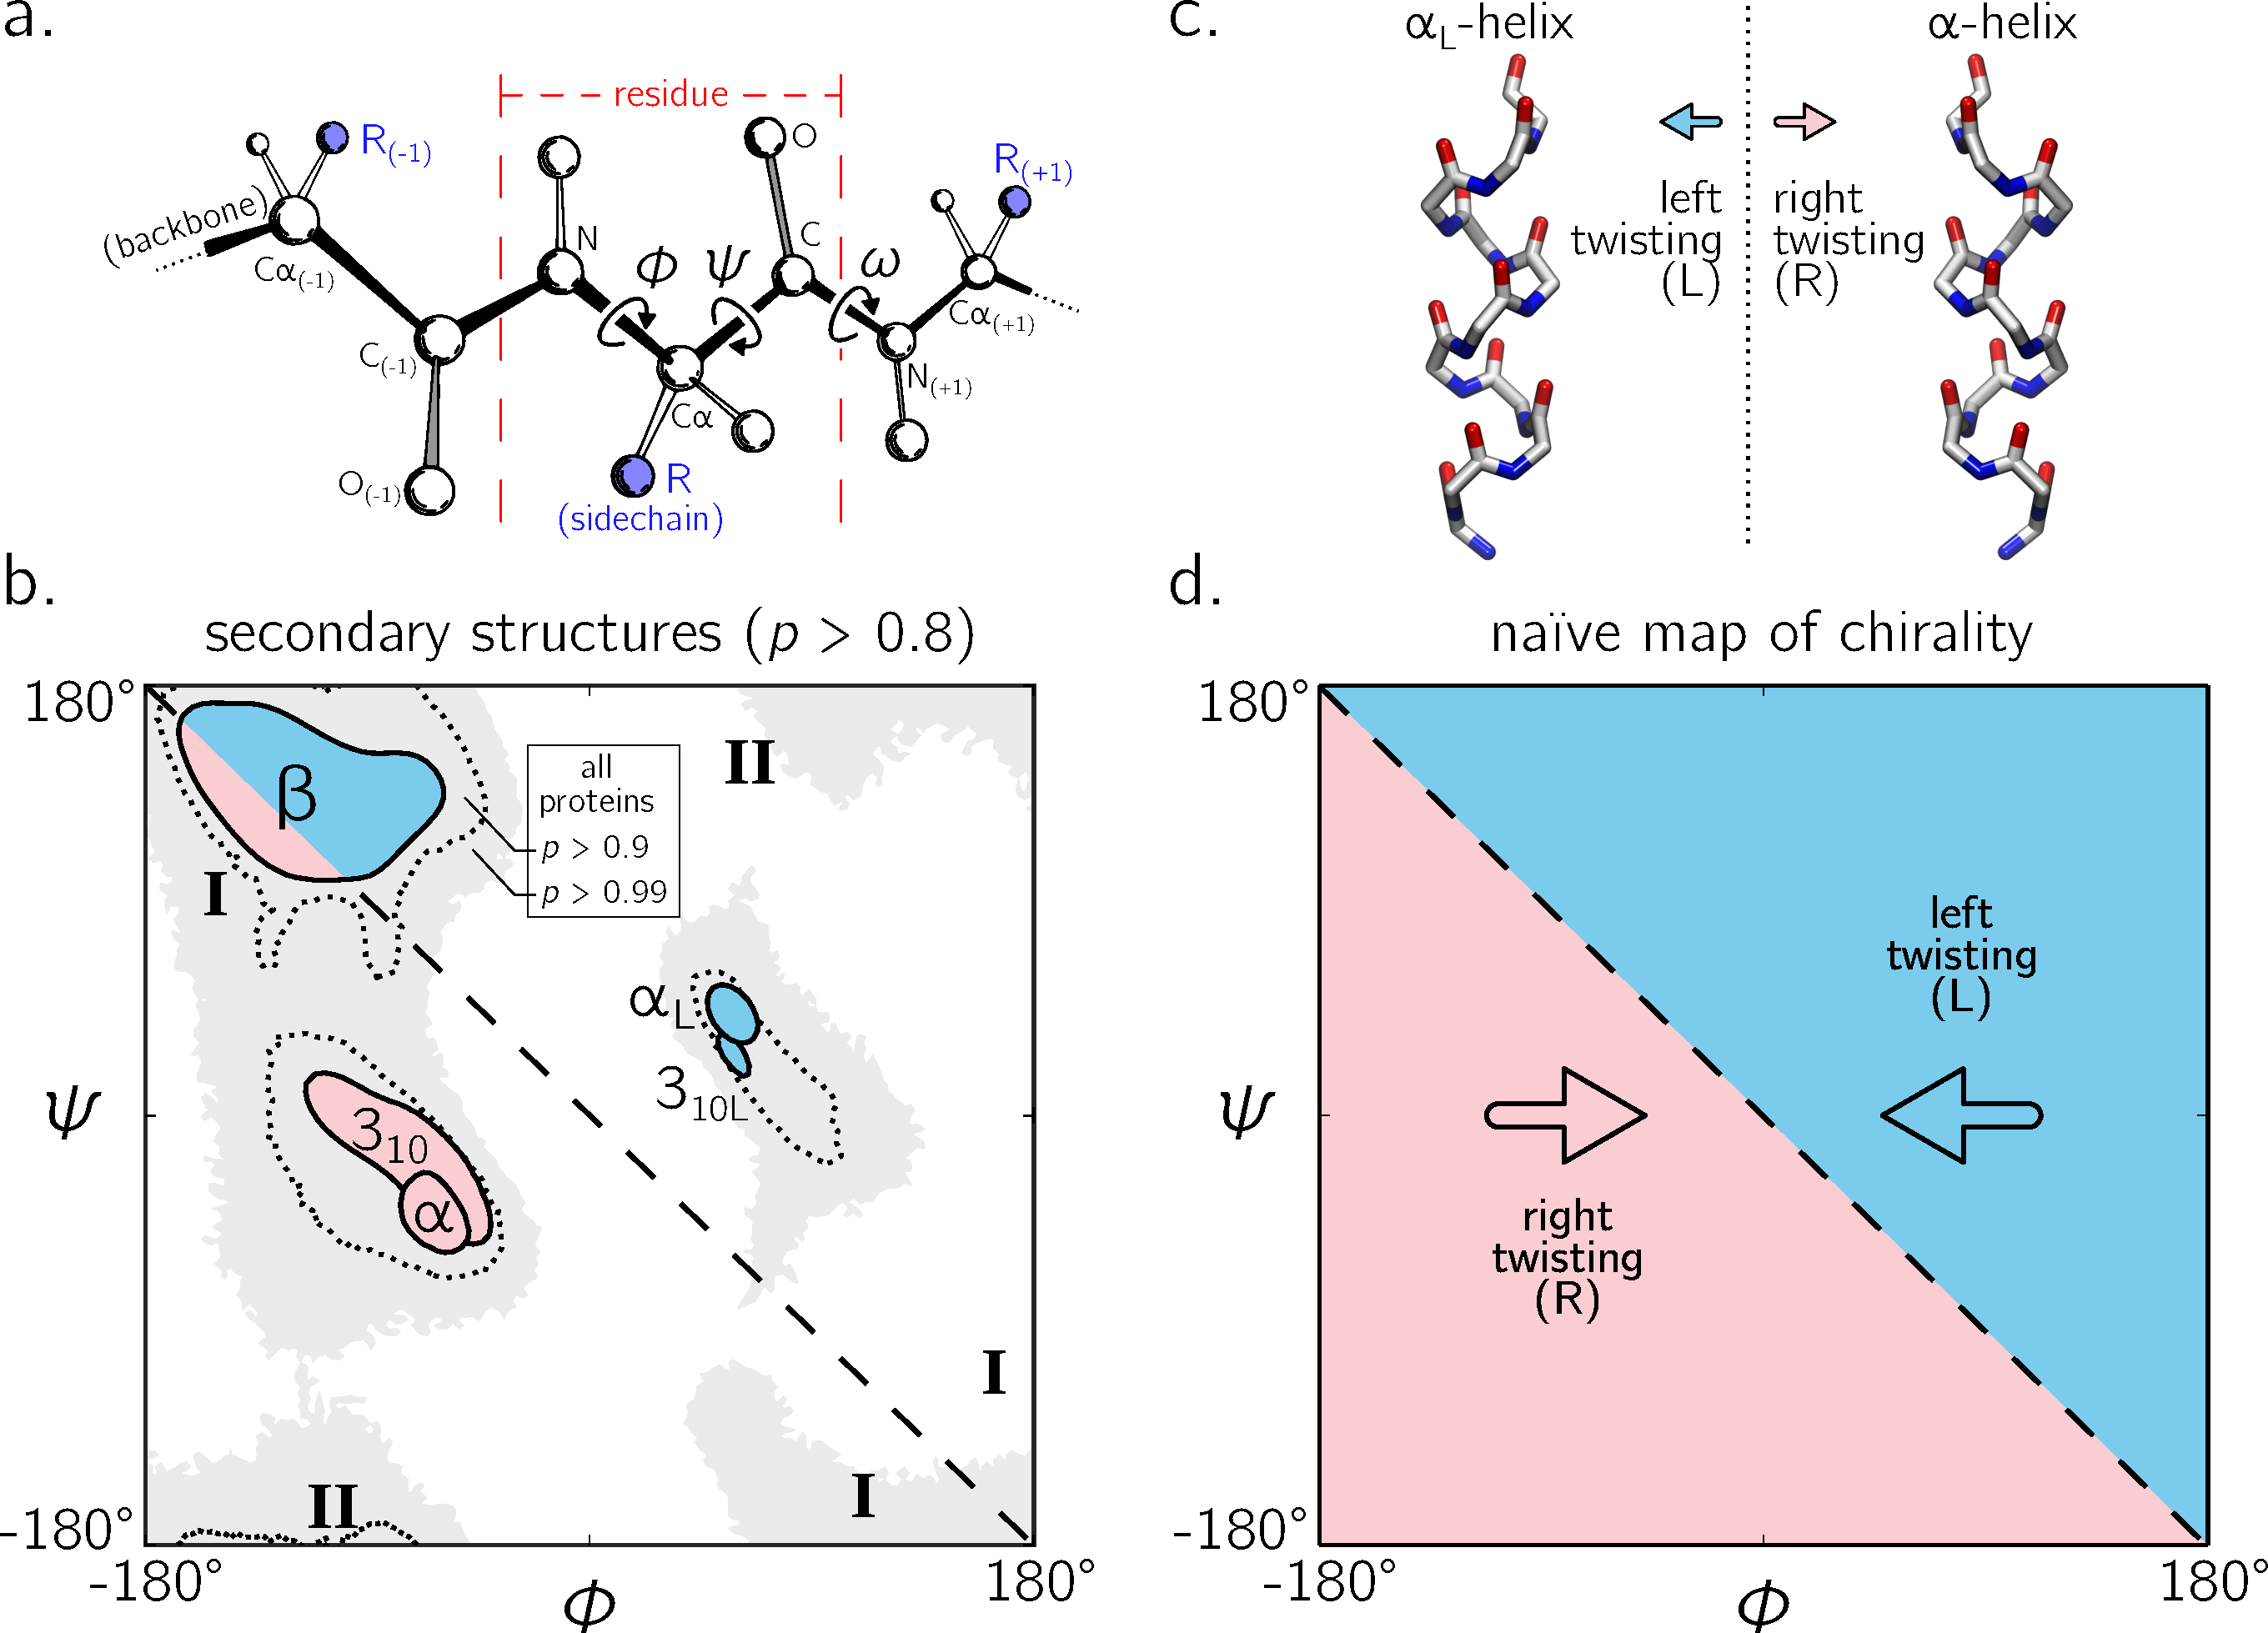
\includegraphics[width=0.8\linewidth]{\figdir/chirality_intro.pdf}
\caption{\label{fig:intro} A peptide is composed of a linear chain of residues (a). Each peptide is structurally distinguished into backbone atoms (connected by dark shaded bonds in a) and sidechain motifs that stick out of each residue's $\upalpha$-carbon ($R$). The structures available to a peptide are mainly due to the dihedral angles $\phi$ and $\psi$ (and in smaller part, $\omega$). For example, repeating a value for $\phi$ and $\psi$ for every residue within a peptide -- i.e., selecting a point on the Ramachandran plot (b) -- results in regular (secondary) structures that then combine to form most globular proteins in the protein databank \citep{Berman2000}. The twist of each perfectly regular secondary structure possesses a distinct chirality: left-handed, or right-handed (examples shown in c); rarely, peptides may be non-chiral or flat (e.g., when $\phi=\psi=\uppi$). As evidenced in (c) the -ve diagonal within the Ramachandran plot (dashed line) divides right-handed peptides from left-handed peptides, which leads to the na{\"i}ve picture of handedness (d). \cite{Zacharias2013} showed that this picture is over simplistic, however an in-depth characterization of the backbone in all regions was not performed, and will be done here for both $cis$ ($\omega=0$) and $trans$ backbones ($\omega=\uppi$).}
\end{figure}

So far, our understanding of the Ramachandran plot has been limited to the secondary structures and loops displayed by proteins \citep{Berman2000,Alberts2002}. Structural biologists are aware that the negatively sloping diagonal (dashed line in \Fig{fig:intro}b; henceforth denoted as the `-ve diagonal') demarcates a change in backbone chirality. For example, the position of the idealized left- and right-handed $\upalpha$-helices (\Fig{fig:intro}c)\footnote{Here and below, all molecular representations are shown in `licorice' form, with the colors red, blue and white representing the oxygen, nitrogen and carbon atoms.} -- respectively denoted as $\upalpha_\textrm{L}$ and $\upalpha$ in \Fig{fig:intro}b -- are on opposite sides of the -ve diagonal\footnote{Note that left- and right-handed backbone twists are respectively associated with the L and D chiralities within the Fisher Projection system and S and R chiralities within the Cahn--Ingold--Prelog system \citep{Cross2013}.}. Additionally, the $\upbeta$-strand exists predominantly on the right of the -ve diagonal, and their backbones are predominantly left-handed [see, e.g., discussions within \cite{Quiocho1977} and \cite{Shaw1977}\footnote{Note that a different metric for handedness in $\beta$ sheets exists today that addresses the handedness of a particular hydrogen bonding network and not the handedness of the participating peptide's backbone. See, e.g., \cite{Schulz1974} and \cite{Chothia1977}.}]. Indeed, all regular/ordered motifs within proteins that lie to the right (or top) of the -ve diagonal are left-handed in backbone twist; as a corollary, all ordered backbones to the left (or under) the -ve diagonal are right-handed in nature (primarily, the $\upalpha$-, $\uppi$- and $3_{10}$-helix; \Fig{fig:intro}b; $\uppi$-helices are not shown due to low frequency in the protein databank). Na{\"i}vely, these observations lead to the hypothesis that the -ve diagonal of the Ramachandran plot separates the left-handed backbones from the right-handed backbones (\Fig{fig:intro}d). While even Pauling and colleagues were cognizant of this general trend in peptide secondary structure [see, e.g., notes on what is now known as the $\upalpha$-sheet; \cite{Pauling1951,Pauling1951a,Pauling1951b}], the picture in \Fig{fig:intro}d is an often assumed one by protein structural biologists, even though its incorrectness is evident in at least one earlier report \citep{Zacharias2013}.

While `twist' chirality in regular protein secondary structures is well understood, peptide mimics -- especially pep\textit{toids} \citep{Sun2013} -- display new secondary structures that fall out of the regions regularly occupied by proteins. Peptoids are distinguished from peptides by the position of each sidechain on the backbone [sidechains are attached to the backbone nitrogen atom rather than the $\upalpha$-carbon; \cite{Sun2013}]. %; \Fig{FigSIpeptoid}). 
Certain peptoids display secondary structures in regions of the Ramachandran plot that are not well characterized  \citep{Sun2013,Goodman2007,Culf2010,Beke2006,Pohl2012,Zuckermann2009,Sun2013}. For example, a `higher-order' peptoid secondary structure -- the $\Sigma$-strand \citep{Mannige2015,Robertson2016} -- samples regions of the Ramachandran plot (`$\textrm{\textbf{I}}$' in \Fig{fig:intro}d) that are not permitted within natural proteins (this is because of the lack of backbone hydrogen bond donors in peptoids). Another secondary structure -- the `$\omega$-strand' \citep{Gorske2016} -- samples similarly `historically uncharted' regions of the Ramachandran plot (`$\textrm{\textbf{II}}$' in \Fig{fig:intro}d). Importantly, handedness plays a crucial part in explaining these new motifs: as one goes along the backbones of these secondary structures, alternating residues occupy equal but opposite backbone twists [for this reason, the $\Sigma$-strand is relatively linear, albeit meandering; \cite{Mannige2015}; \cite{MannigeKunduWhitelam2016}].

In light of these new secondary structures, and in anticipation of the discovery of additional (higher-order) secondary structures, we chose to perform a detailed study into how regular backbones twist in each region of the Ramachandran plot. This question builds on a previous report that discussed handedness in all-$trans$-backbones \citep{Zacharias2013}, and would complete our understanding of a very basic component of biochemistry (handedness and twist of a backbone). An additional aim is to completely dispel the na{\"i}ve view in \Fig{fig:intro}d.

\begin{figure}[t!]
\mbox{}\hfill
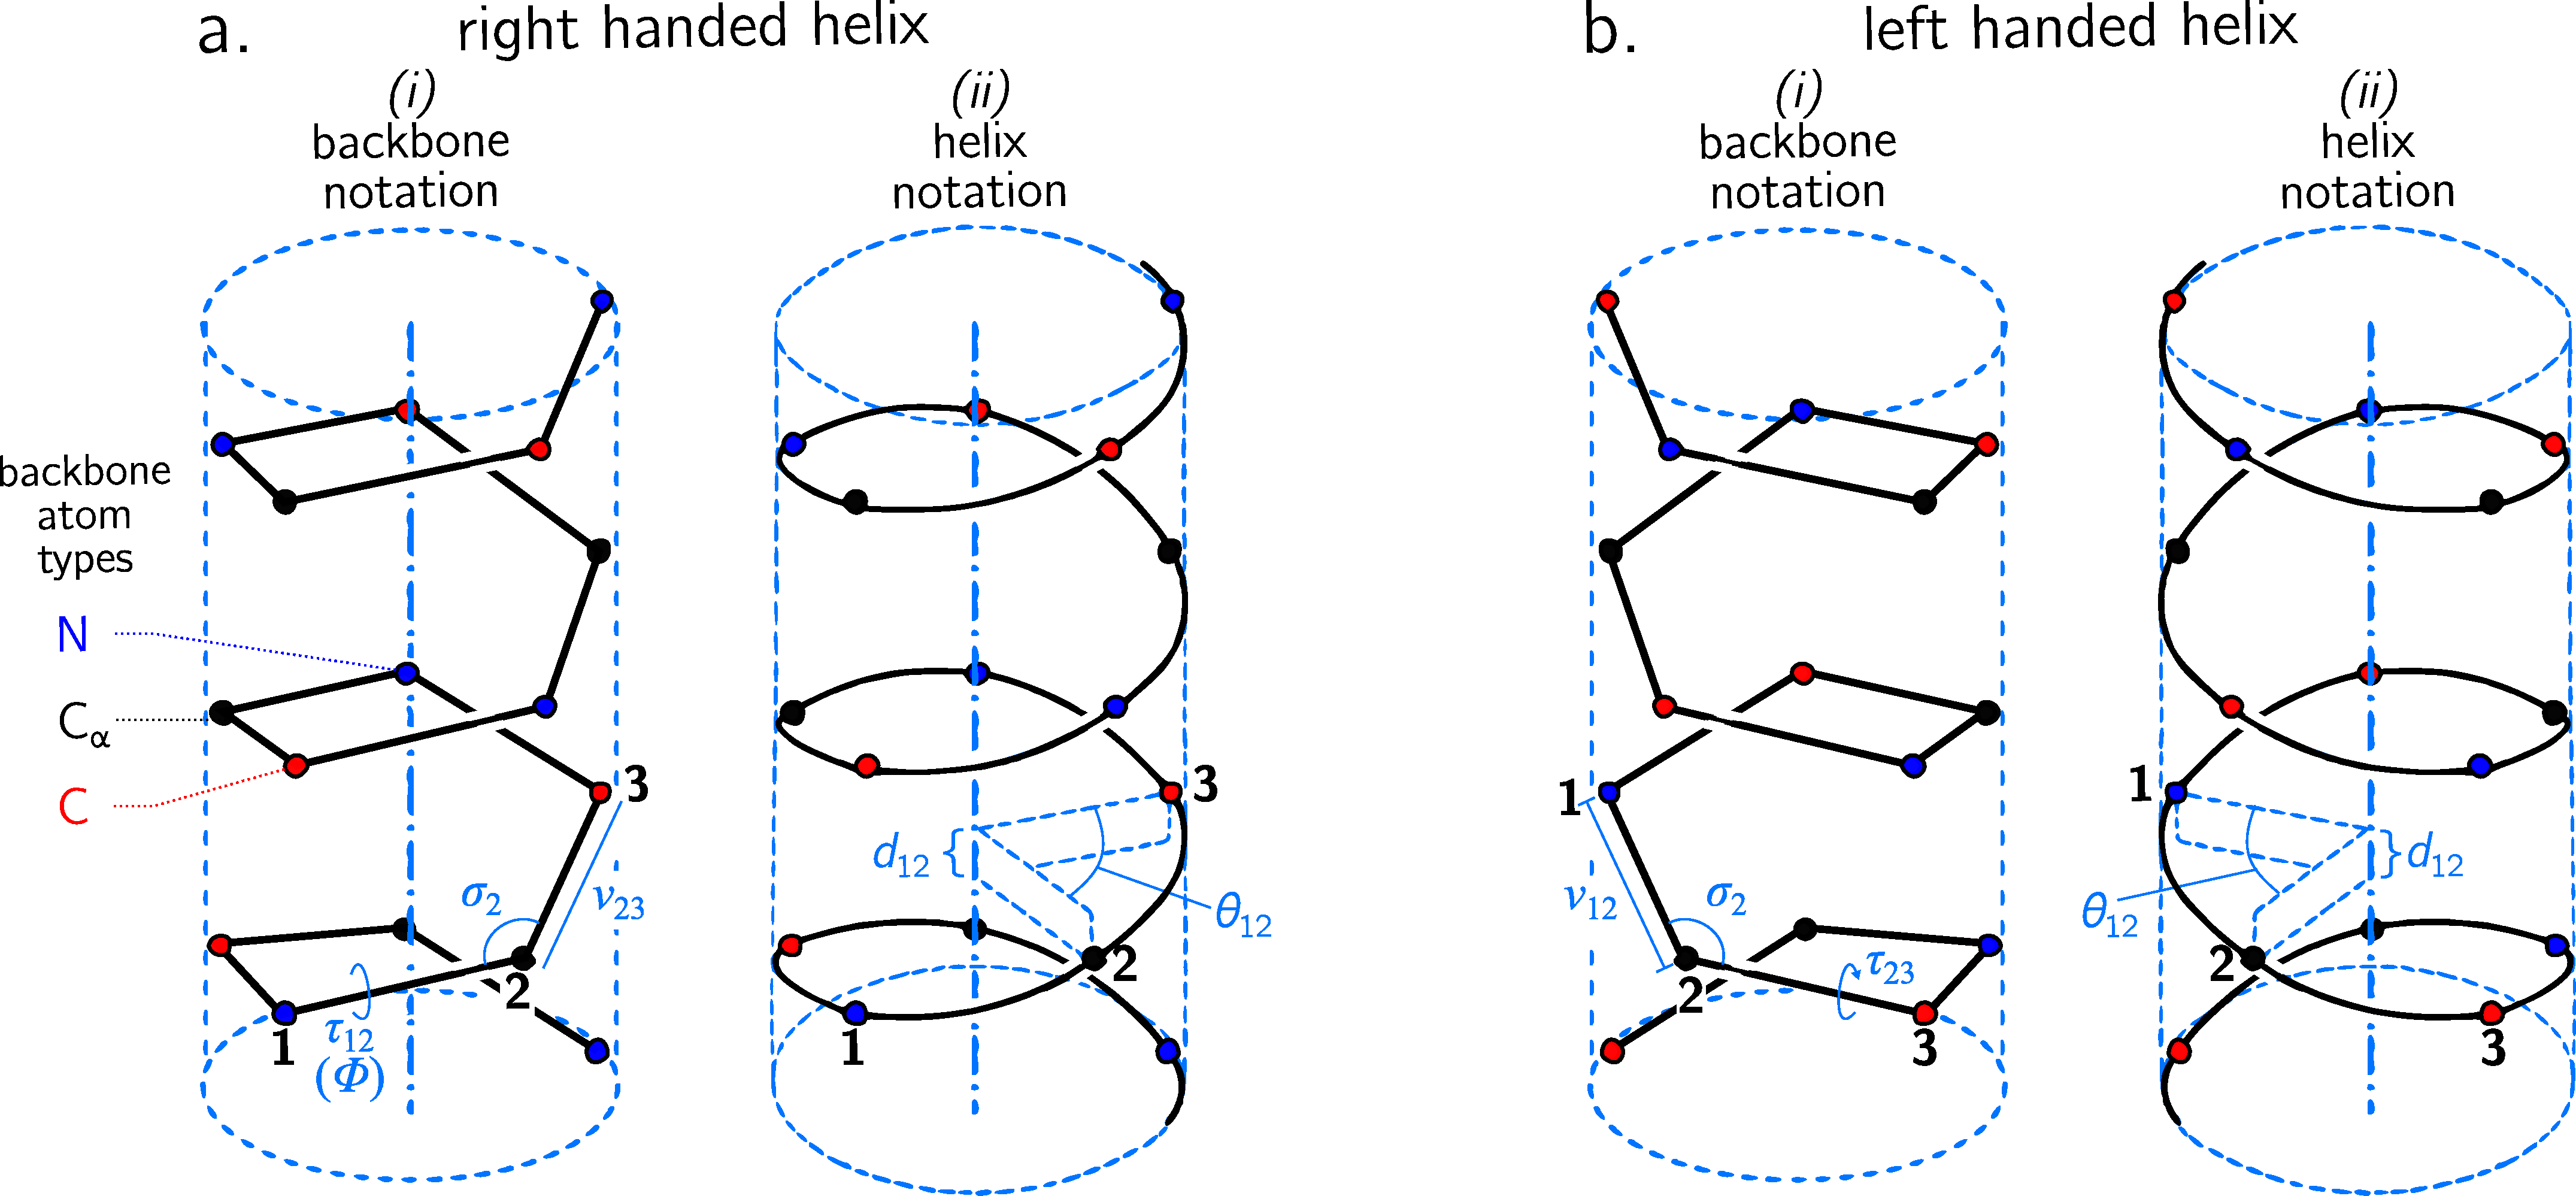
\includegraphics[width=0.9\textwidth]{\figdir/helix_peptide.pdf}
\hfill\mbox{}\hfill\mbox{}\newline
  \caption{Internal coordinate \textit{(i)} and helical coordinate \textit{(ii)} representations of right-handed (a) and left-handed (b) regular backbones. Internal coordinates are a function of bond lengths (e.g., $v_{12}$), angles ($\sigma_{2}$), and dihedral angles ($\tau_{12}$), while helical coordinates are a function of displacement along the helical axis ($d_{12}$), angular displacement in the plane perpendicular to the helical axis ($\theta_{12}$) and shortest distance of an  atom from the helical axis ($\rho$; not shown). Representations are derived from Fig.~1 in \citep{Shimanouchi1955}.
\label{fig:helix}}
\end{figure}

\section*{Methods}
All methods and materials required to produce this manuscript are freely available at \url{https://github.com/ranjanmannige/backbone_chirality}.

\subsection*{Deriving measures for backbone handedness}
Numerous metrics for molecular chirality and handedness have so far been discussed \citep{Harris1999}. For example, metrics for chirality have been introduced that focus on vector orientations \citep{Kwiecinska2005,Gruziel2013}, optical activity \citep{Osipov1995}, and molecular shape \citep{Ferrarini1998}. However, we will focus on a simpler metric for chirality associated with an idealized helix within which all atoms of the backbone sits \citep{Shimanouchi1955,Miyazawa1961,Zacharias2013}. We do this because any {\em regular} backbone can be associated with a specific helix\footnote{Indeed, the word `helix' has a broader meaning that comes from the Greek word $\check\epsilon\lambda\iota\xi$ that means `twisted, curved'; \cite{Liddell1894}.}, and, as we will discuss below, helices have handedness baked into the equations. We will first introduce the use of helical coordinates (and how peptides may be treated in such contexts), after which we will show how some parameters within the helical coordinate system (namely $d$ and $\theta$) may be combined to describe a physically unambiguous meaning of handedness of a backbone's twist.

\subsection*{Describing a regular backbone as a helix.} Interest in how a backbone may be represented as a helix emerged shortly after the first secondary structures were introduced \citep{Pauling1951,Pauling1951a,Pauling1951b}. \cite{Shimanouchi1955} had derived a set of equations that fit a platonic helix to the atoms within a {\it regularly arranged} backbone. Here, a `regular' backbone  indicates that each tunable parameter within a unit or `residue' -- say a particular dihedral angle -- remains the same for all residues. \Fig{fig:helix} describes an arbitrary peptide backbone that may be represented either using internal coordinates \textit{(i)} or helical coordinates \textit{(ii)}. 

Internal coordinates are associated with (stereo)chemical terms: bond lengths ($v_{ij}$) between adjacent atoms $i$ and $j$, bond angles ($\sigma_{i}$) between the two backbone bonds adjacent to atom $i$, and dihedral or torsion angles ($\tau_{ij}$), which are associated with the bond $i-j$ and the atoms preceding and succeeding these atoms. Helical coordinates (\Fig{fig:helix}\textit{(ii)}) are described using measures of vertical displacement ($d$; this is related to the pitch of a platonic helix), angular displacement ($\theta$) and the radius of the helix ($\rho$; not shown in \Fig{fig:helix})\footnote{\cite{Miyazawa1961} also reported a helix parameter related to $\theta$ and $d$ -- the radius ($\rho$) of the helix (Eqn.~38 in that report) -- which will not be discussed here, as its meaning with regards to handedness is redundant.}. Given that there are three atoms associated with a residue (\Fig{fig:intro}a), $d$ and $\theta$, which are per-residue values, are described in terms of distances ($d_{hk}$) and angles ($\theta_{hk}$) between adjacent atoms, where  $\left(h,k\right)\in\{\left(\textrm{n}_i,\upalpha_{i}\right), \left(\upalpha_{i},\textrm{c}_i\right), \left(\textrm{n}_i,\textrm{c}_{i+1}\right)\}$. Here, 
$\textrm{n}_i$, $\upalpha_i$, and $\textrm{c}_i$ are the backbone nitrogen, $\upalpha$-carbon, and carbonyl carbon atoms (\Fig{fig:intro}a), and the index $i$ (or $i+1$) indicates residue position. 

The notation used by \cite{Shimanouchi1955} were in terms of matrices, which were then simplified by \cite{Miyazawa1961} into trigonometric terms\footnote{Interestingly, the formalisms described by \cite{Miyazawa1961} and \cite{Shimanouchi1955} apply to repeating linear polymers of arbitrary complexity; therefore, these formalisms can be applied to even novel protein mimics that do not conserve the number of atoms within the backbone \citep{Kandakov2013}, such as $\upbeta$-peptides.}. In particular, \cite{Miyazawa1961} noted that the total residue-residue vertical displacement ($d$) and angular displacement ($\theta$) may be retrieved using the following two equations.

\begin{align}
\cos\left(\frac{\theta}{2}\right) =&\cos\left(\frac{+\phi+\psi+\omega}{2}\right) \sin\left(\frac{\sigma_\textrm{n}}{2}\right) \sin\left(\frac{\sigma_\upalpha}{2}\right) \sin\left(\frac{\sigma_\textrm{c}}{2}\right) \nonumber \\
                                  -&\cos\left(\frac{+\phi-\psi+\omega}{2}\right) \sin\left(\frac{\sigma_\textrm{n}}{2}\right) \cos\left(\frac{\sigma_\upalpha}{2}\right) \cos\left(\frac{\sigma_\textrm{c}}{2}\right) \nonumber \\
                                  -&\cos\left(\frac{+\phi+\psi-\omega}{2}\right) \cos\left(\frac{\sigma_\textrm{n}}{2}\right) \sin\left(\frac{\sigma_\upalpha}{2}\right) \cos\left(\frac{\sigma_\textrm{c}}{2}\right) \nonumber \\
                                  -&\cos\left(\frac{-\phi+\psi+\omega}{2}\right) \cos\left(\frac{\sigma_\textrm{n}}{2}\right) \cos\left(\frac{\sigma_\upalpha}{2}\right) \sin\left(\frac{\sigma_\textrm{c}}{2}\right)
                                  \label{eqn:theta}
\end{align}
\begin{align} 
d \sin\left(\frac{\theta}{2}\right) = & \left(+v_{\textrm{n,}\upalpha}+v_{\upalpha\textrm{,c}}+v_\textrm{c,n}\right)\sin\left(\frac{+\phi+\psi+\omega}{2}\right)\sin\left(\frac{\sigma_\textrm{n}}{2}\right)\sin\left(\frac{\sigma_\upalpha}{2}\right)\sin\left(\frac{\sigma_\textrm{c}}{2}\right)\nonumber \\
                                    - & \left(+v_{\textrm{n,}\upalpha}-v_{\upalpha\textrm{,c}}+v_\textrm{c,n}\right)\sin\left(\frac{+\phi-\psi+\omega}{2}\right)\sin\left(\frac{\sigma_\textrm{n}}{2}\right)\cos\left(\frac{\sigma_\upalpha}{2}\right)\cos\left(\frac{\sigma_\textrm{c}}{2}\right)\nonumber \\
                                    - & \left(+v_{\textrm{n,}\upalpha}+v_{\upalpha\textrm{,c}}-v_\textrm{c,n}\right)\sin\left(\frac{+\phi+\psi-\omega}{2}\right)\cos\left(\frac{\sigma_\textrm{n}}{2}\right)\sin\left(\frac{\sigma_\upalpha}{2}\right)\cos\left(\frac{\sigma_\textrm{c}}{2}\right)\nonumber \\
                                    - & \left(-v_{\textrm{n,}\upalpha}+v_{\upalpha\textrm{,c}}+v_\textrm{c,n}\right)\sin\left(\frac{-\phi+\psi+\omega}{2}\right)\cos\left(\frac{\sigma_\textrm{n}}{2}\right)\cos\left(\frac{\sigma_\upalpha}{2}\right)\sin\left(\frac{\sigma_\textrm{c}}{2}\right)
                                    \label{eqn:d}
\end{align}
Here, subscripts `$\textrm{n}$', `$\upalpha$', and `$\textrm{c}$' respectively refer to the backbone nitrogen, $\upalpha$-carbon and carbonyl carbon atoms; $v_{ij}$ refers to the distance between adjacent atoms $i$ and $j$; $\sigma_i$ refers to the angle between the adjacent bonds that have $i$ as the common atom. Finally, $\phi$, $\psi$, and $\omega$ represent the traditional  symbols for backbone dihedral angles, which may be otherwise denoted as $\tau_{\textrm{n},\upalpha}$, $\tau_{\upalpha,\textrm{c}}$, and $\tau_{\textrm{c},\textrm{n}(+1)}$, respectively. Given that backbone bond lengths and angles are generally less tunable when compared to dihedral angles, we can keep them fixed. Using revised values for the bond angles and lengths\footnote{Values used here are also used by \cite{Zacharias2013}. These values are: \\% and were reported within \citep{Engh1991,Engh2006}: \\
$v_{\textrm{n,}\upalpha} = 1.459\textrm{\AA}$,\hfill
$v_{\upalpha\textrm{,c}} = 1.525\textrm{\AA}$, \hfill
$v_\textrm{c,n(+1)} = 1.336\textrm{\AA}$, \hfill
$\sigma_\upalpha = 111.0$,\hfill
$\sigma_\textrm{c} = 117.2^\circ$, \hfill and \hfill
$\sigma_\textrm{n} = 121.7^\circ$. \hfill \\
For reference, \cite{Miyazawa1961} originally used the following values:\\ 
$v_{\textrm{n,}\upalpha} = 1.470\textrm{\AA}$,\hfill
$v_{\upalpha\textrm{,c}} = 1.530\textrm{\AA}$,\hfill 
$v_\textrm{c,n(+1)} = 1.320\textrm{\AA}$, \hfill
$\sigma_\upalpha = 110.0$,\hfill
$\sigma_\textrm{c} = 114.0$, \hfill and \hfill
$\sigma_\textrm{n} = 123.0$.}, 
we arrive at equations for $\theta$ and $d$ that are purely a function of the backbone dihedral angles. In particular, \cite{Miyazawa1961} set $\omega=\uppi$ and used preset values for bond angles and lengths to arrive at a simpler equation for $trans$ backbones. An updated version of this equation follows \citep{Zacharias2013}.
\begin{align}
\label{eqn:theta_trans}
\cos\left(\frac{\theta}{2}\right) =-&~0.8235~\sin\left(\frac{\phi+\psi}{2}\right) 
                                    +0.0222~\sin\left(\frac{\phi-\psi}{2}\right),\\
\label{eqn:d_trans}
d \sin\left(\frac{\theta}{2}\right) =&~2.9986~\cos\left(\frac{\phi+\psi}{2}\right)
                                      -0.6575~\cos\left(\frac{\phi-\psi}{2}\right).
\end{align}

This equation is especially relevant to peptides as they occur predominantly in $trans$ conformations ($\omega=\uppi$). However, given the prevalence of $cis$ backbones in peptide mimics such as peptoids \citep{Mirijanian2014,Gorske2016}, for completeness, we report the corresponding relationships for a $cis$ backbone ($\omega=0$) below.
\begin{align}
\label{eqn:theta_cis}
\cos\left(\frac{\theta}{2}\right) =&~0.4052~\cos\left(\frac{\phi+\psi}{2}\right)
                                    -0.4932~\cos\left(\frac{\phi-\psi}{2}\right), \\
\label{eqn:theta_d}
d \sin\left(\frac{\theta}{2}\right) = &~2.3093~\sin\left(\frac{\phi+\psi}{2}\right)
                                       +0.0028~\sin\left(\frac{\phi-\psi}{2}\right).
\end{align}

\begin{figure}[t!]
\centering
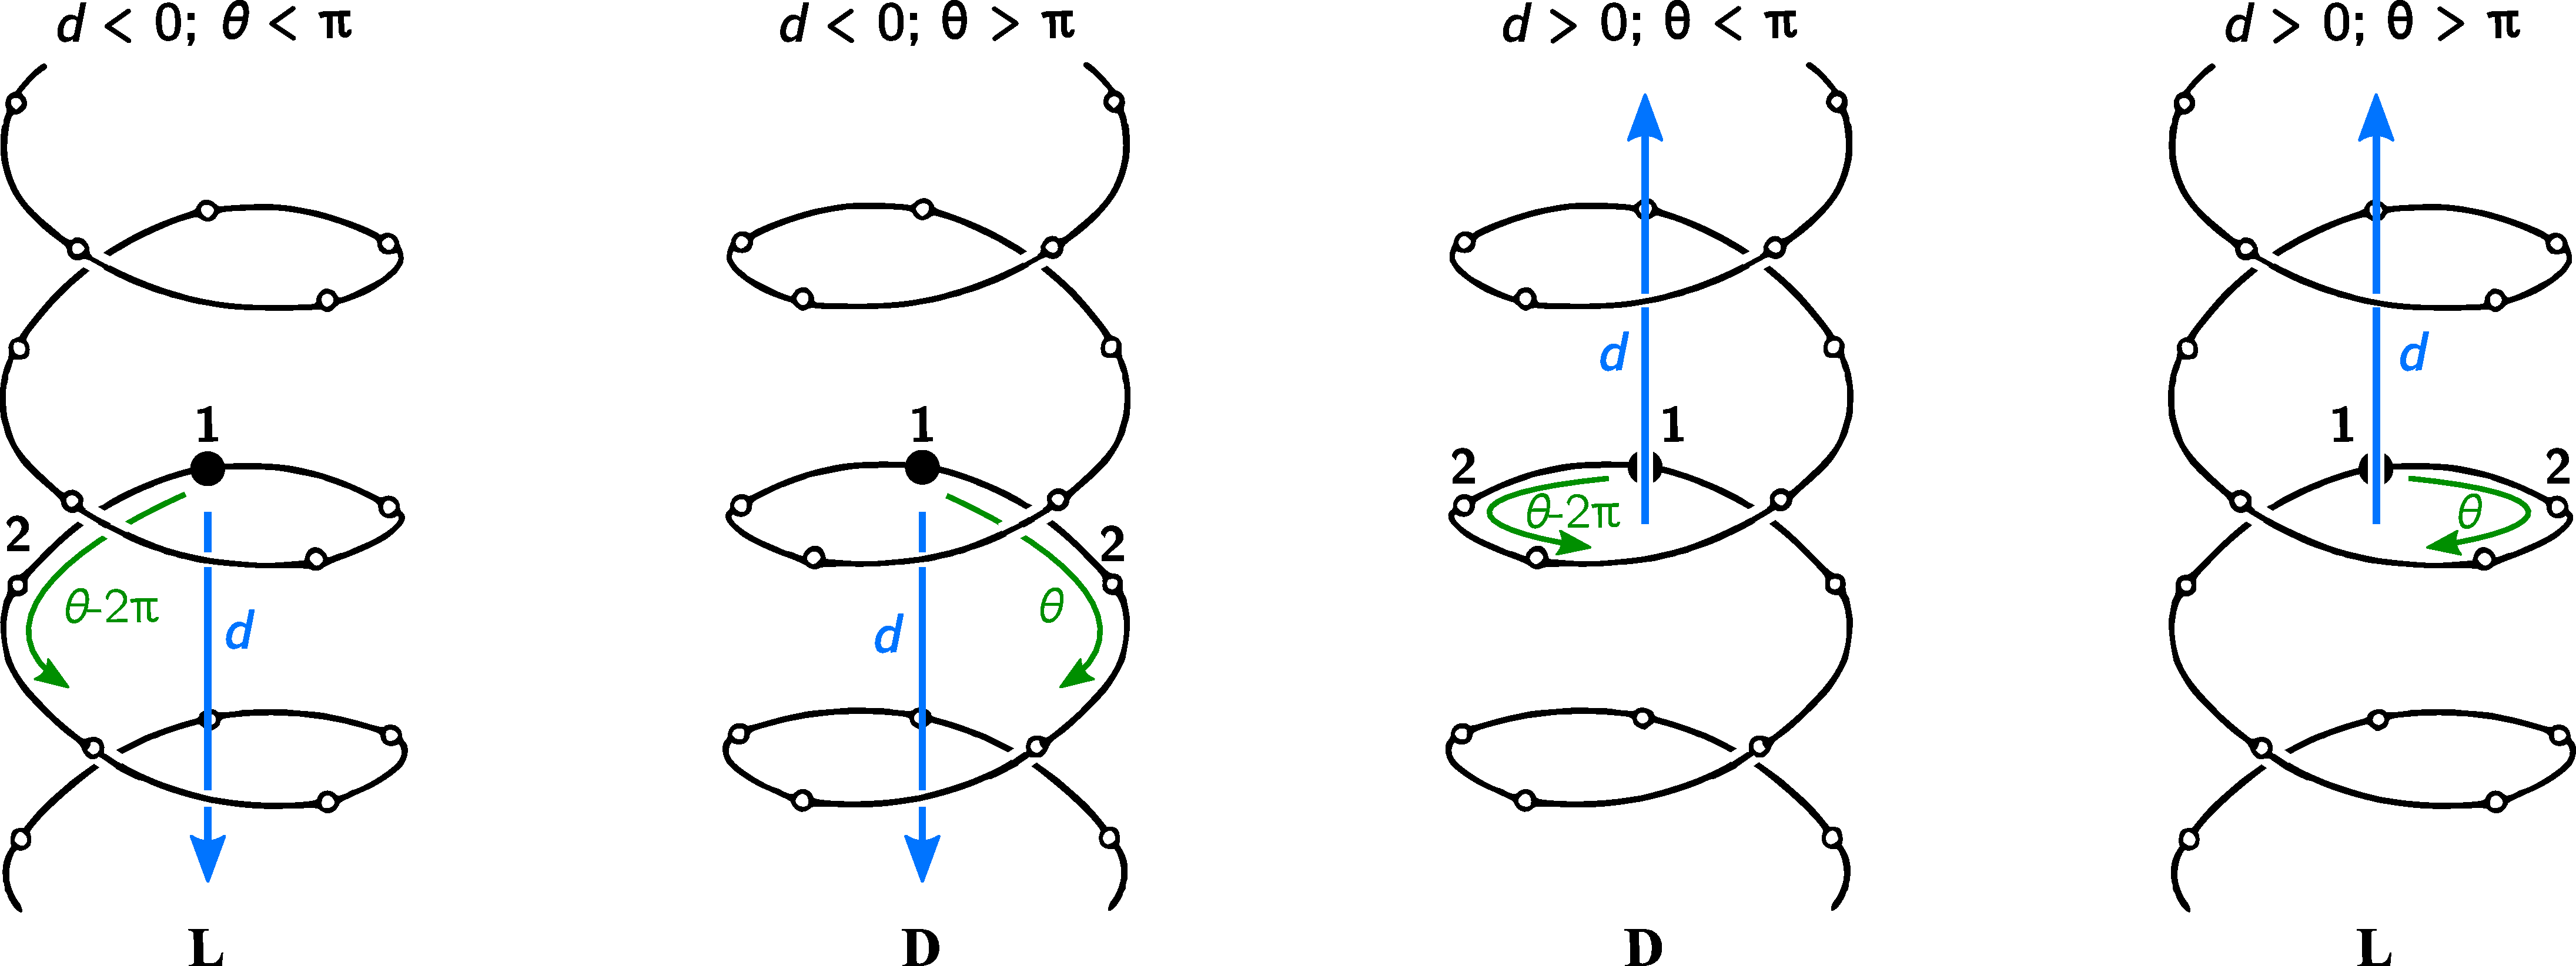
\includegraphics[width=0.85\linewidth]{\figdir/helix_handedness.pdf}
\caption{\label{fig:helix_handedness} The handedness of a helix is a function of angular displacement perpendicular to the helical axis ($\theta$; green curved arrows) and linear displacement along the helical axis $d$ (blue, vertical arrows). Here, the left- and right-handed twists are respectively referred to as $\textbf{L}$ and $\textbf{D}$ (shown at the bottom), as per the Fisher Projection system \citep{Cross2013}.}
\end{figure}

\subsection*{An equation for backbone handedness.} 
The helical parameters $d$ and $\theta$ host a wealth of information. For example, $d=0$ indicates all atoms of a particular type (e.g., all $\upalpha$-carbons) are in the same plane. For any fixed value of $d$, the backbone is least curved when $\theta=\uppi$; similarly, for any fixed value of $\theta$, the backbone is most tightly wound when $\theta$ assumes the value of $d=0$. \cite{Zacharias2013} observed that $\theta$ and $d$ are also instrumental in describing backbone handedness. We describe this relationship first by words and pictures (\Fig{fig:helix_handedness}), and then in equation form.

The relationship between $d$, $\theta$ and  handedness is shown in \Fig{fig:helix_handedness}. While $\theta$ indicates the extent to which a backbone is curved, the handedness of a backbone is dependent on both $\theta$ and $d$, because the sign of $d$ provides a frame of reference for interpreting $\theta$. In particular, if $d$ is positive, then $\theta < \uppi$ indicates right handedness, while $\theta > \uppi$ indicates a left-handed helix. However, if $d$ is negative, then the manner in which the helix is `built' reverses (\Fig{fig:helix_handedness}), and $\theta>\uppi$ indicates left-handedness, while $\sin(\theta)<\uppi$ indicates right-handedness.

Given these relationships, we provide the following, simple, metric for backbone handedness that depends on the sign of $d$ and the value of $\theta$:
\begin{equation}\label{eqn:chi}
\chi = \frac{d}{|d|}\frac{\uppi-\theta}{\uppi}
\end{equation}
Here, $\chi \in \{-1,\ldots,1\}$ is negative (or positive) when the overall twist of the backbone is left (or right) handed\footnote{A similar but not identical outcome could be obtained if we use the equation $\chi' = \frac{d}{|d|}\sin(\theta)$.}.

\subsection*{Alternative measures of handedness.} 
Two estimates for handedness -- $\chi_1$ and $\chi_2$ -- used to validate the derived measure of chirality $\chi$ (\Eqn{eqn:chi}) were previously used by \cite{Kwiecinska2005} and \cite{Gruziel2013}, respectively. The equations are: \begin{equation} \label{eqn:chi1}
\chi_1 = \frac{1}{N}\sum_{i = 2}^{N-2} \frac{(\textit{\textbf{v}}_{i-1} \times \textit{\textbf{v}}_{i})\cdot \textit{\textbf{v}}_{i+1}}{\textit{v}_{i-1} \textit{v}_{i} \textit{v}_{i+1}},
\end{equation}
\begin{equation}\label{eqn:chi2}
\displaystyle \chi_2 = \frac{1}{\uppi N}\sum_{i = 2}^{N-2}
 \textrm{arctan2}\left (\textit{v}_i \textit{\textbf{v}}_{i-1} \cdot \textit{\textbf{v}}_i \times \textit{\textbf{v}}_{i+1},\textit{\textbf{v}}_{i-1}\times \textit{\textbf{v}}_i \cdot \textit{\textbf{v}}_i\times \textit{\textbf{v}}_{i+1} \right ).
\end{equation}

%$\chi_1$, was used previously as a measure of helix twist handedness 
Here, $N$ is the peptide length, $i$ is the peptide residue number and the position of each $\upalpha$-carbon is $\textit{\textbf{N}}_i$, with vector $\textit{\textbf{v}}_{k} \equiv \textit{\textbf{N}}_{k+1} - \textit{\textbf{N}}_{k}$. 
%Vector $\textit{\textbf{v}}_{ij} \equiv \textit{\textbf{N}}_{i} - \textit{\textbf{N}}_{j}$ and $\textit{\textbf{v}}_{k} \equiv \textit{\textbf{v}}_{k+1,k} = \textit{\textbf{N}}_{k+1} - \textit{\textbf{N}}_{k}$. 
The scalar component of the vector $\textit{\textbf{v}}_i$ is denoted as $\textit{v}_i$. 
%Each scalar in the denominator within the summand (e.g. $\textit{v}_i$) indicates the distance between neighboring alpha carbons, which is $\sim$3\ang and $\sim$3.85\ang for backbones whose amide dihedral angles respectively are $cis$ ($\omega\approx0$) and $trans$ ($\omega\approx\uppi$). If we know that the backbone amide is either all-$cis$ or all-$trans$, then the denominator can be simplified to $\textit{v}_i^3$.
In both metrics, the average peptide backbone handedness has range $[-1,1]$\footnote{Although \Eqn{eqn:chi2} in \cite{Gruziel2013} is not normalized by $\uppi$ and has the range $[-\uppi,\uppi]$.}. Values deviating more from 0 are more chiral (or `twisted' or `handed'), and left-handed twists are negative while right-handed twists are positive. Only $\upalpha$-carbon atom positions are used for the calculation. 

%\begin{equation}\label{eqn:chi3}
%\displaystyle \chi_2 = \frac{4!}{3N^4} \sum_{i,j,k,l \in \textit{\textbf{N}}} \frac{((\textit{\textbf{v}}_{ij} \times \textit{\textbf{v}}_{kl}) \cdot \textit{\textbf{v}}_{il}) (\textit{\textbf{v}}_{ij} \cdot \textit{\textbf{v}}_{jk}) (\textit{\textbf{v}}_{jk} \cdot \textit{\textbf{v}}_{kl})} {\left(\textit{v}_{ij} \textit{v}_{jk} \textit{v}_{kl}\right)^2 \textit{v}_{il}}.
%\end{equation}
%$\chi_2$, of arbitrary range $[-\lambda,\lambda]$, is known as the chirality index $G_{0S}$ in \cite{Solymosi2002} and \cite{Neal2003}. $(i,j,k,l)$ are exhaustive permutations of $\{1,2,\ldots,N\}$.

While \Eqn{eqn:chi} is purely analytical and does not need structures to be computationally generated, \Eqns{eqn:chi1} and~\ref{eqn:chi2} do. In order to use these equations, peptides (poly-glycines) of arbitrary length were generated using the Python-based PeptideBuilder library \citep{Matthew2013}. %\footnote{As we are dealing with regular peptides, peptide length need only be greater than 4 residues.}. 
Analysis was performed using BioPython \citep{Cock2009} and Numerical Python \citep{VanDerWalt2011}. Ramachandran plots that describe chirality (e.g., \Fig{fig:chi}a) were generated using a grid spacing of $\phi,\psi \in \{-180,-178,\ldots,178,180\}$.

\section*{Discussion}

\begin{figure}[t!]
\begin{adjustwidth}{-1in}{0in} % Comment out/remove adjustwidth environment if table fits in text column.
\centering
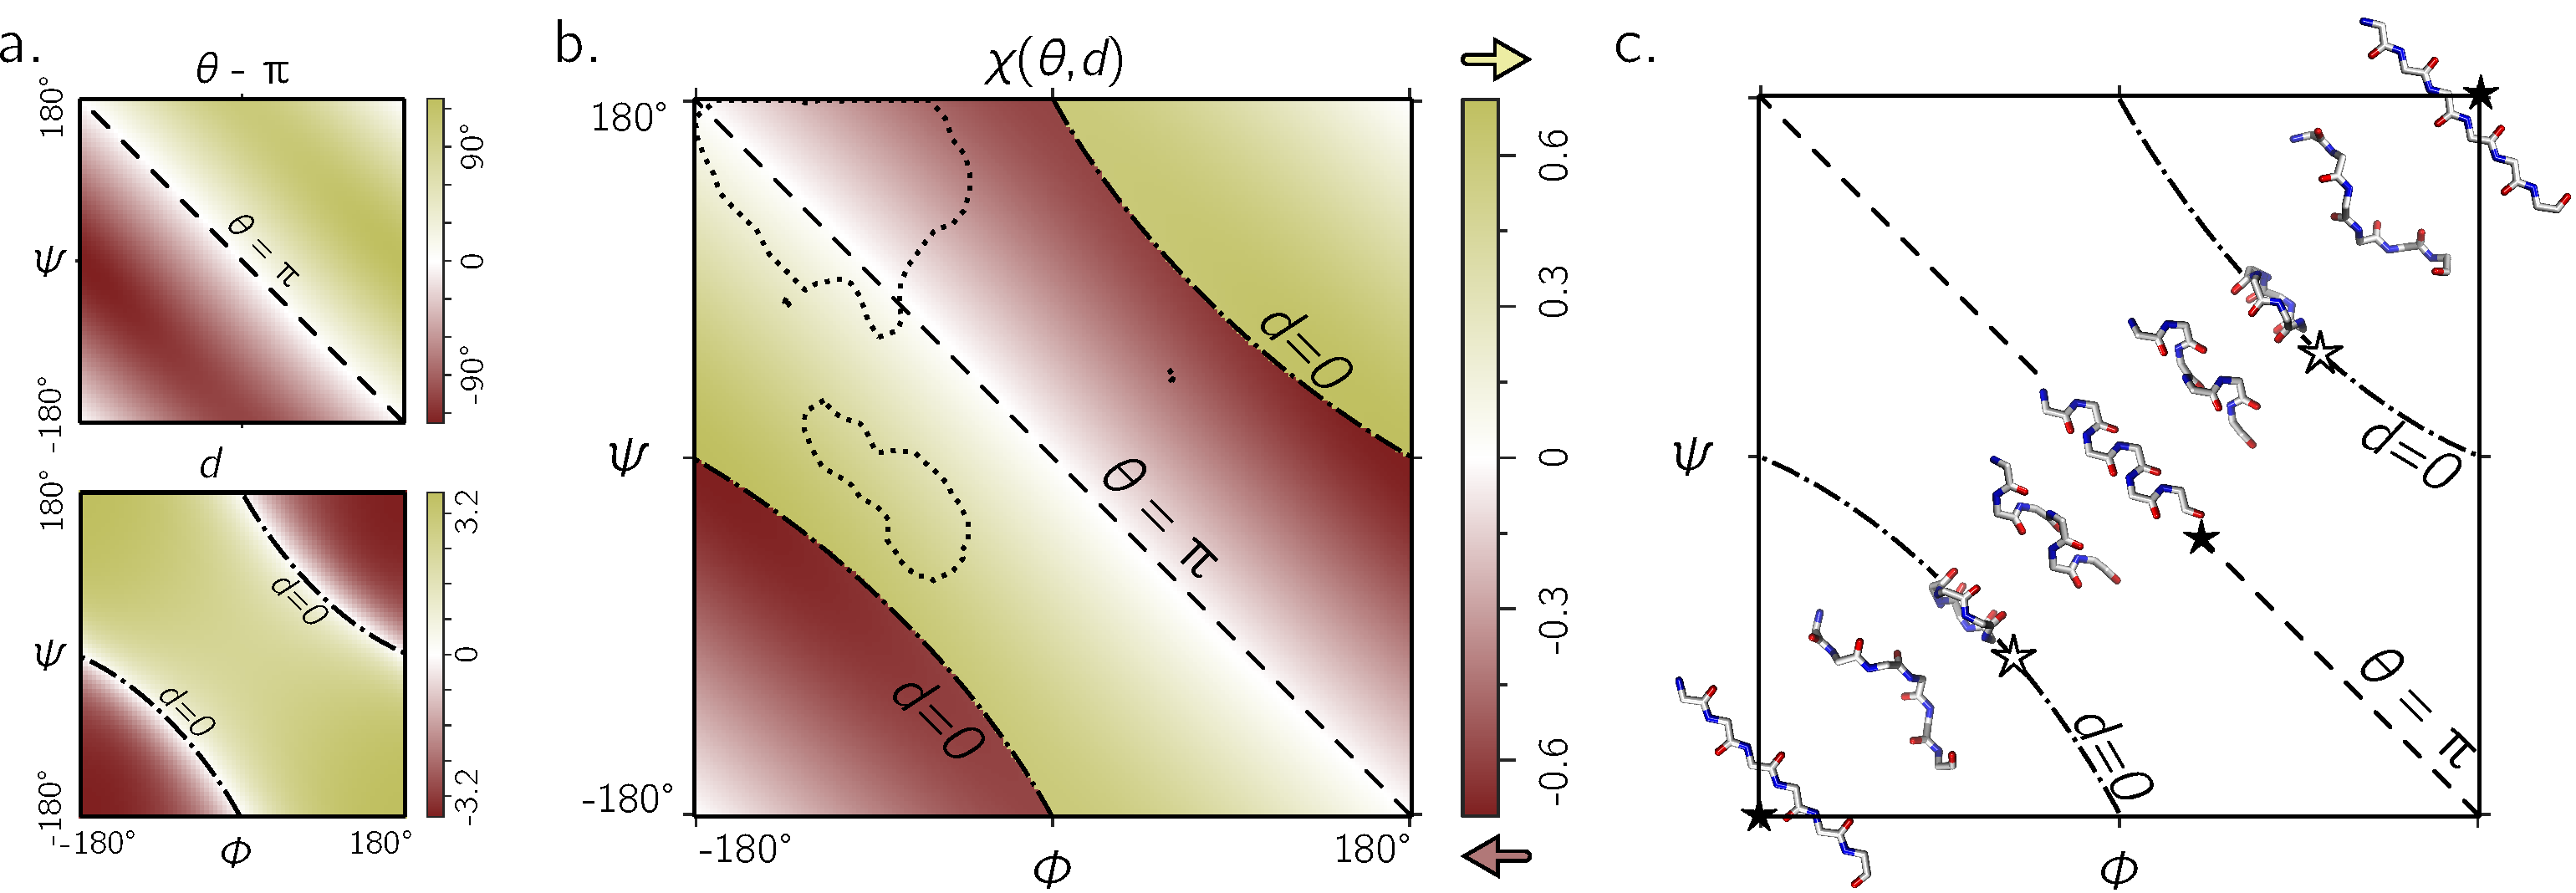
\includegraphics[width=\linewidth]{\figdir/chi_snapshots.pdf}
\caption{\label{fig:chi} The chirality of an ordered $trans$ peptide within the Ramachandran plot. Panel (a) displays the relationship between backbone parameters $(\phi,\psi)$ and the associated helix parameters of curvature $\theta-\uppi$ (top; \Eqn{eqn:theta}) and pitch $d$ (bottom; \Eqn{eqn:d}). The boundaries, $\theta = \uppi$ (`\protect\dashedrule') and $d=0$ (`\protect\dotdashedrule'), correspond to backbones that are equally flat, but which are respectively optimally extended and curved (see discussion in text). As shown in \Fig{fig:helix_handedness}, the handedness of a helix is a function of these two variables ($\chi$; \Eqn{eqn:chi}). Panel (b) is a map of backbone chirality ($\chi$) as a function of $\phi$ and $\psi$. 
This map shows that the na{\"i}ve expectation of handedness in a Ramachandran plot (\Fig{fig:intro}d) is inaccurate.  Interestingly, our na{\"i}ve expectations (\Fig{fig:intro}d) would be upheld if we were only to have sampled regions of the Ramachandran plot dominated by known proteins (a; regions enclosed by `\protect\dottedrule'). An example of the behavior of one `slice' of (b) is shown in (c). Each snapshot represents a peptide backbone that is either in a distinct region of handedness or at a boundary. Secondary structure statistics were obtained from \cite{MannigeKunduWhitelam2016}. %Given that this is previously reported, we have not provided code for this procedure within the GitHub repository. As per \cite{MannigeKunduWhitelam2016}, $\upalpha$-helices, $3_{10}$-helices and $\upbeta$-sheets were identified using the DSSP algorithm \citep{Zhao2005,Kabsch1983,Joosten2011} and sourced from protein structures within the 40\% non-redundant database provided by the Structural Classification of Proteins or SCOP (Release 2.03; \cite{Fox2014}). The polyproline II helix statistics were obtained from segments within 16,535 proteins annotated by PolyprOnline \citep{Chebrek2014} to contain three or more residues of the secondary structure.
}
\end{adjustwidth}
\end{figure}

\subsection*{Relevance of $\bm \theta$ and $\bm d$.}
The helical parameters $d$ and $\theta$ respectively refer to a displacement along the helical axis and an angular displacement in a plane perpendicular to the helical axis (\Fig{fig:helix_handedness}).  \Fig{fig:chi}a describes the behavior of $d$ and $\theta-\uppi$ as a function of $\phi$ and $\psi$ (assuming an all-$trans$ backbone; $\omega=0$). 
As discussed previously, both $d$ and $\theta$ are structurally important: $d=0$ codes for backbones that are both flat and optimally extended (for a fixed $theta$), while $\theta=\uppi$ codes for backbones that are both flat and optimally collapsed or curved (for a fixed $d$); these ideas are further discussed below in context of $trans$ backbones. 

Two possible definitions of backbone `flatness' are possible: flatness at a residue level and flatness at the atomic level. In the former, all atoms of the same {\em type} are coplanar (examples of atom types are backbone nitrogen, carbonyl carbon, $\upalpha$-carbon, or even sidechain $\upbeta$-carbon). In the latter, {\em all} atoms within the backbone are coplanar. We choose the former definition as the relevant definition of flatness, as we are only concerned about the residue-by-residue behavior of the peptide. 

Given basic combination guidelines (\Fig{fig:helix_handedness}), $\theta$ and $d$ combines into $\chi$ (\Eqn{eqn:chi}) to define the handedness of a backbone. In absence of handedness, when $\chi=0$, we have an achiral or flat backbone. 

\begin{figure}[t!]
\begin{adjustwidth}{-1in}{0in} % Comment out/remove adjustwidth environment if table fits in text column.
\centering
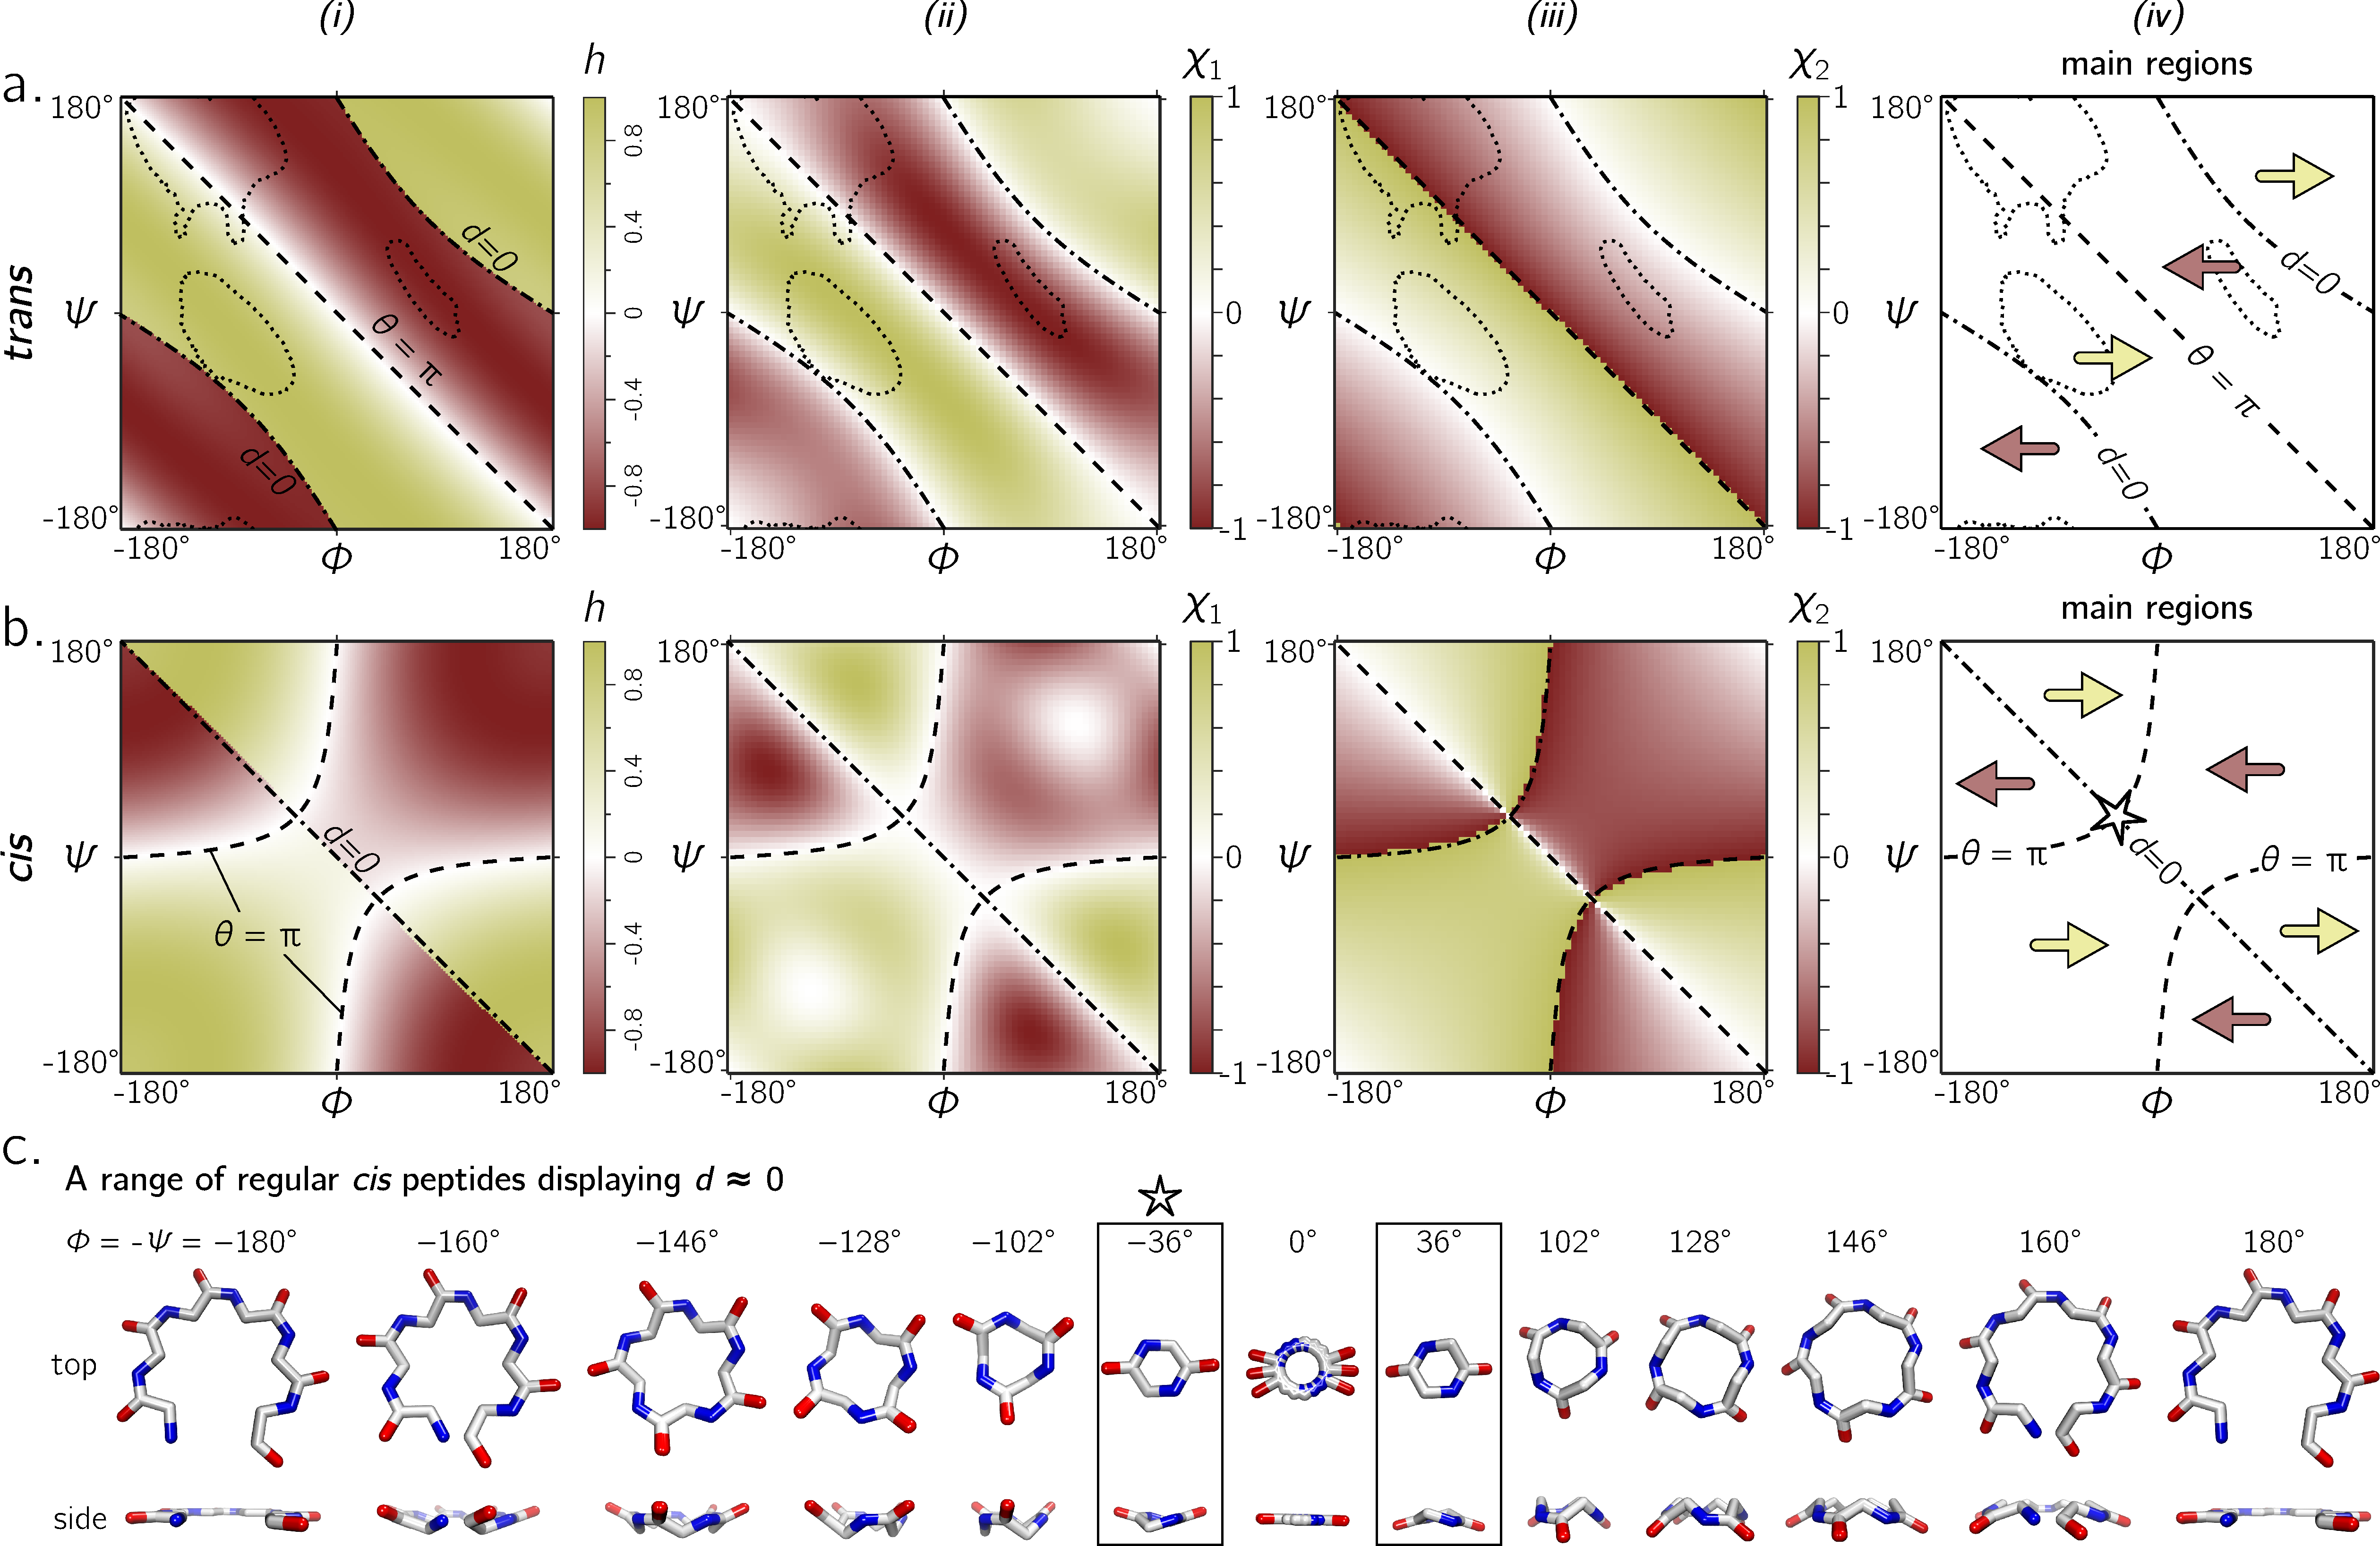
\includegraphics[width=\linewidth]{\figdir/various_chis.pdf}
\caption{Panels (a) and (b) describe the handedness of backbones twists whose amide dihedral angles are $trans$ ($\omega=\uppi$) and $cis$ ($\omega=0$), respectively. Column \textit{(i)} describes handedness calculated using $\chi$ (\Eqn{eqn:chi}), which does not require structures to be computationally generated. Columns \textit{(ii)} and \textit{(iii)} respectively show vector-based estimates of backbone handedness -- $\chi_1$ (\Eqn{eqn:chi1}) and $\chi_2$ (\Eqn{eqn:chi2}) -- which are calculated from computationally generated peptides (see Methods). Regions of left- and right-handedness are identical for all measures of handedness \textit{(i--iii)}. This general map of how handedness is distributed within the Ramachandran plot is shown in \textit{(iv)}. 
As in \Fig{fig:chi}, `\protect\dashedrule' and `\protect\dotdashedrule' respectively correspond to $\theta = \uppi$ and $d=0$.
\label{fig:chi_all}}
\end{adjustwidth}
\end{figure}

\subsection*{Handedness within \textit{trans} backbones.}

\Fig{fig:chi}b is a complete description of the chirality of an all-$trans$ peptide backbone. It describes the behavior of backbone handedness as a measure of $\phi$ and $\psi$, while \Fig{fig:chi}c describes some structures at relevant regions within the Ramachandran plot. When $d=0$ (`\FiveStarOpen'), then each residue is at the same `altitude', i.e., the helix is perfectly flat and curved. Note that any path on the Ramachandran plot that transitions from negative to positive $d$ will encounter an infinitesimal region in its path that is $d=0$: it therefore does not appear white as would be expected for a region where $\chi=0$, but as a sharp transition from one handedness to the other. When $\theta=\uppi$, then the backbone is also flat (see `\FiveStar' in \Fig{fig:chi}c); however, these backbones are also linear (i.e., each atom type is co\textit{linear}). In short: Within the Ramachandran plot, $d=0$ (`\protect\dotdashedrule') and $\chi=\uppi$ (`\protect\dashedrule') code for {\it flat} backbones that are respectively either optimally collapsed (at a given $\theta$) or optimally extended (at a given $d$). We later show how these simple rules may be combined to make conjectures about novel secondary and tertiary structures.

\Fig{fig:chi_all}a shows that the equation for $\chi$ match other metrics for handedness and chirality \citep{Kwiecinska2005,Gruziel2013}. In particular, \Fig{fig:chi_all}a displays the Ramachandran plot colored by $\chi$ \textit{(i)} next to estimates calculated using $\chi_1$ (\textit{(ii)}; \Eqn{eqn:chi1}) and $\chi_2$ (\textit{(iii)}; \Eqn{eqn:chi2}). Each panel describes identical regions of left and right handedness, which is shown as a cartoon in \textit{(iv)}. However, given that $\chi_1$ and $\chi_2$ are estimates, their exact values differ from the primary metric for handedness ($\chi$) provided here.

\subsection*{Handedness within \textit{cis} backbones.}
In the same vein as \Fig{fig:chi_all}a, \Fig{fig:chi_all}b displays $\chi$, $\chi_1$ and $\chi_2$ as a function of $\phi$ and $\psi$ for all-$cis$ backbones. Too our recollection, this is the first complete description of chirality of an all-$cis$ backbone ($\omega=0$). Interestingly, the boundaries for $d=0$ and $\theta=\uppi$ switch in $cis$ backbones, with the -ve diagonal and curved boundaries being caused by $d$ and $\theta$, respectively. Additionally, \Fig{fig:chi_all}a reiterates the idea that $cis$ peptides are quite different when compared to $trans$ peptides: the regions and boundaries of left- and right-handedness within the Ramachandran plot differ for $cis$ versus $trans$. Finally, points on the $cis$ map ($\phi=\pm36^\circ$, $\psi=\mp36^\circ$) exist where $d=0$ {\em and} $\theta=\uppi$. An example of a six-residue peptide is shown:\newline
\mbox{}\hfill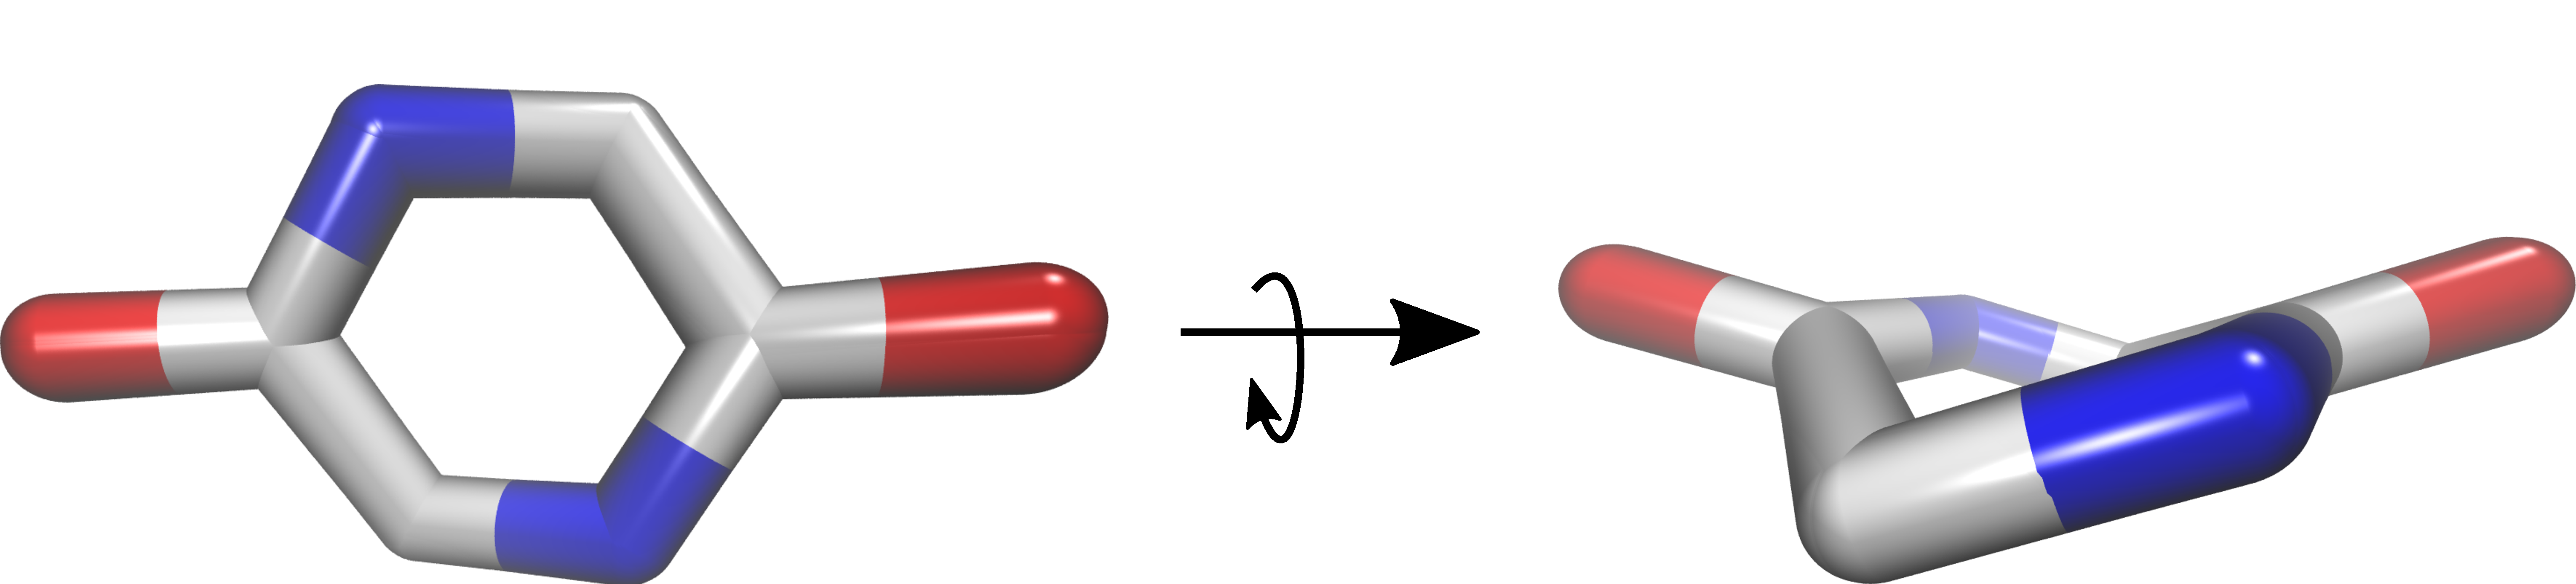
\includegraphics[width=0.3\linewidth]{\figdir/cis_phi_-36.pdf}\hfill\mbox{}\newline
This appears to be almost a contradiction, because $d=0$ indicates the most curved backbone at a fixed $\theta$, and $\theta=\uppi$ indicates the most linear backbone at a fixed $d$. Of course, this structure would never be possible, since many atoms overlap. However, such a structure (one with $d=0$ and $\theta=\uppi$) is not possible in $trans$ peptides, even in theory, because the boundaries associated with $d=0$ and $\theta=\uppi$ will never intersect (\Fig{fig:chi_all}a). 

\subsection*{[$\bm{-\uppi}$,$\bm{\uppi}$] or [$\bm{0}$,$\bm{2\uppi}$]: which frame of reference to use?} 
In structural biology, $\phi$ and $\psi$ within the Ramachandran plot has been historically set to range between the values $[-\uppi,\uppi]$ radians [see, e.g., textbooks by \cite{Berg2006} and \cite{Alberts2002}]. However, \cite{Ramachandran1963} had originally used the range of $[0,2\uppi]$. Today, the range $[-\uppi,\uppi]$ is used predominantly by structural biologists \citep{Laskowski1993,Laskowski2003,Zacharias2013}, while some have turned to $[0,2\uppi]$ as the norm \citep{Nemethy1966,Voelz2011}. 

Given the periodicity of the Ramachandran plot, these differences do not make any difference scientifically; however the value of the Ramachandran plot is undeniably relative to its boundaries: it is a map of important features of proteins and their relatives in context to the various regions, quadrants, and diagonals in the map. The ramachandran plot's value lies in being able to convey large amounts of information in easy to read logo- or picto-grams. For that reason, switching the map from one range to another means that two norms and two types of scientists will not be able to converse as seamlessly.

Therefore, the following question must arise: which range is able to convey more information with the least amount of work? \Fig{fig:other_chis_skewed} shows the behavior of a $trans$ backbone (a,b) $cis$ backbone (c,d) in the two frames of reference. From (a) and (b) it is evident that general trends in the map for $trans$ backbones remain the same in both frames of reference: the negative diagonal ($\sigma=\uppi$) locally separates right from left-handed regions, while the curved line ($d=0$) -- which also separates handedness -- also appears to be in generally the same regions (albeit inverted in curvature). The $cis$ backbones, however, look dramatically different in the two frames of reference: the diagonal appears meaningfully separates handedness when the plot ranges from $0$ o $2\uppi$ (d), while the range $[-\uppi,\uppi]$ separates handedness in a more complicated manner (c). For this reason, purely when looking at handedness,  and especially in the case of $cis$ backbones, the range $0$ o $2\uppi$ appears to be more meaningful.
%\cite{Laskowski1993,Laskowski2003,Zacharias2013,MannigeKunduWhitelam2016}
%The Ramachandran plot has been displayed to students of structural biology primarily in the range of $[-\uppi,\uppi]$\cite{Berg2006,Alberts2002}. 
%range between $-\uppi$ and $\uppi$\footnote{An angle $\zeta$ can be wrapped within the range $[-180,180)$ using $\zeta' = - 180 + (\zeta + 180) \% (360)$, where $\%$ represents the modulus function.}



\begin{figure}[t!]
\centering
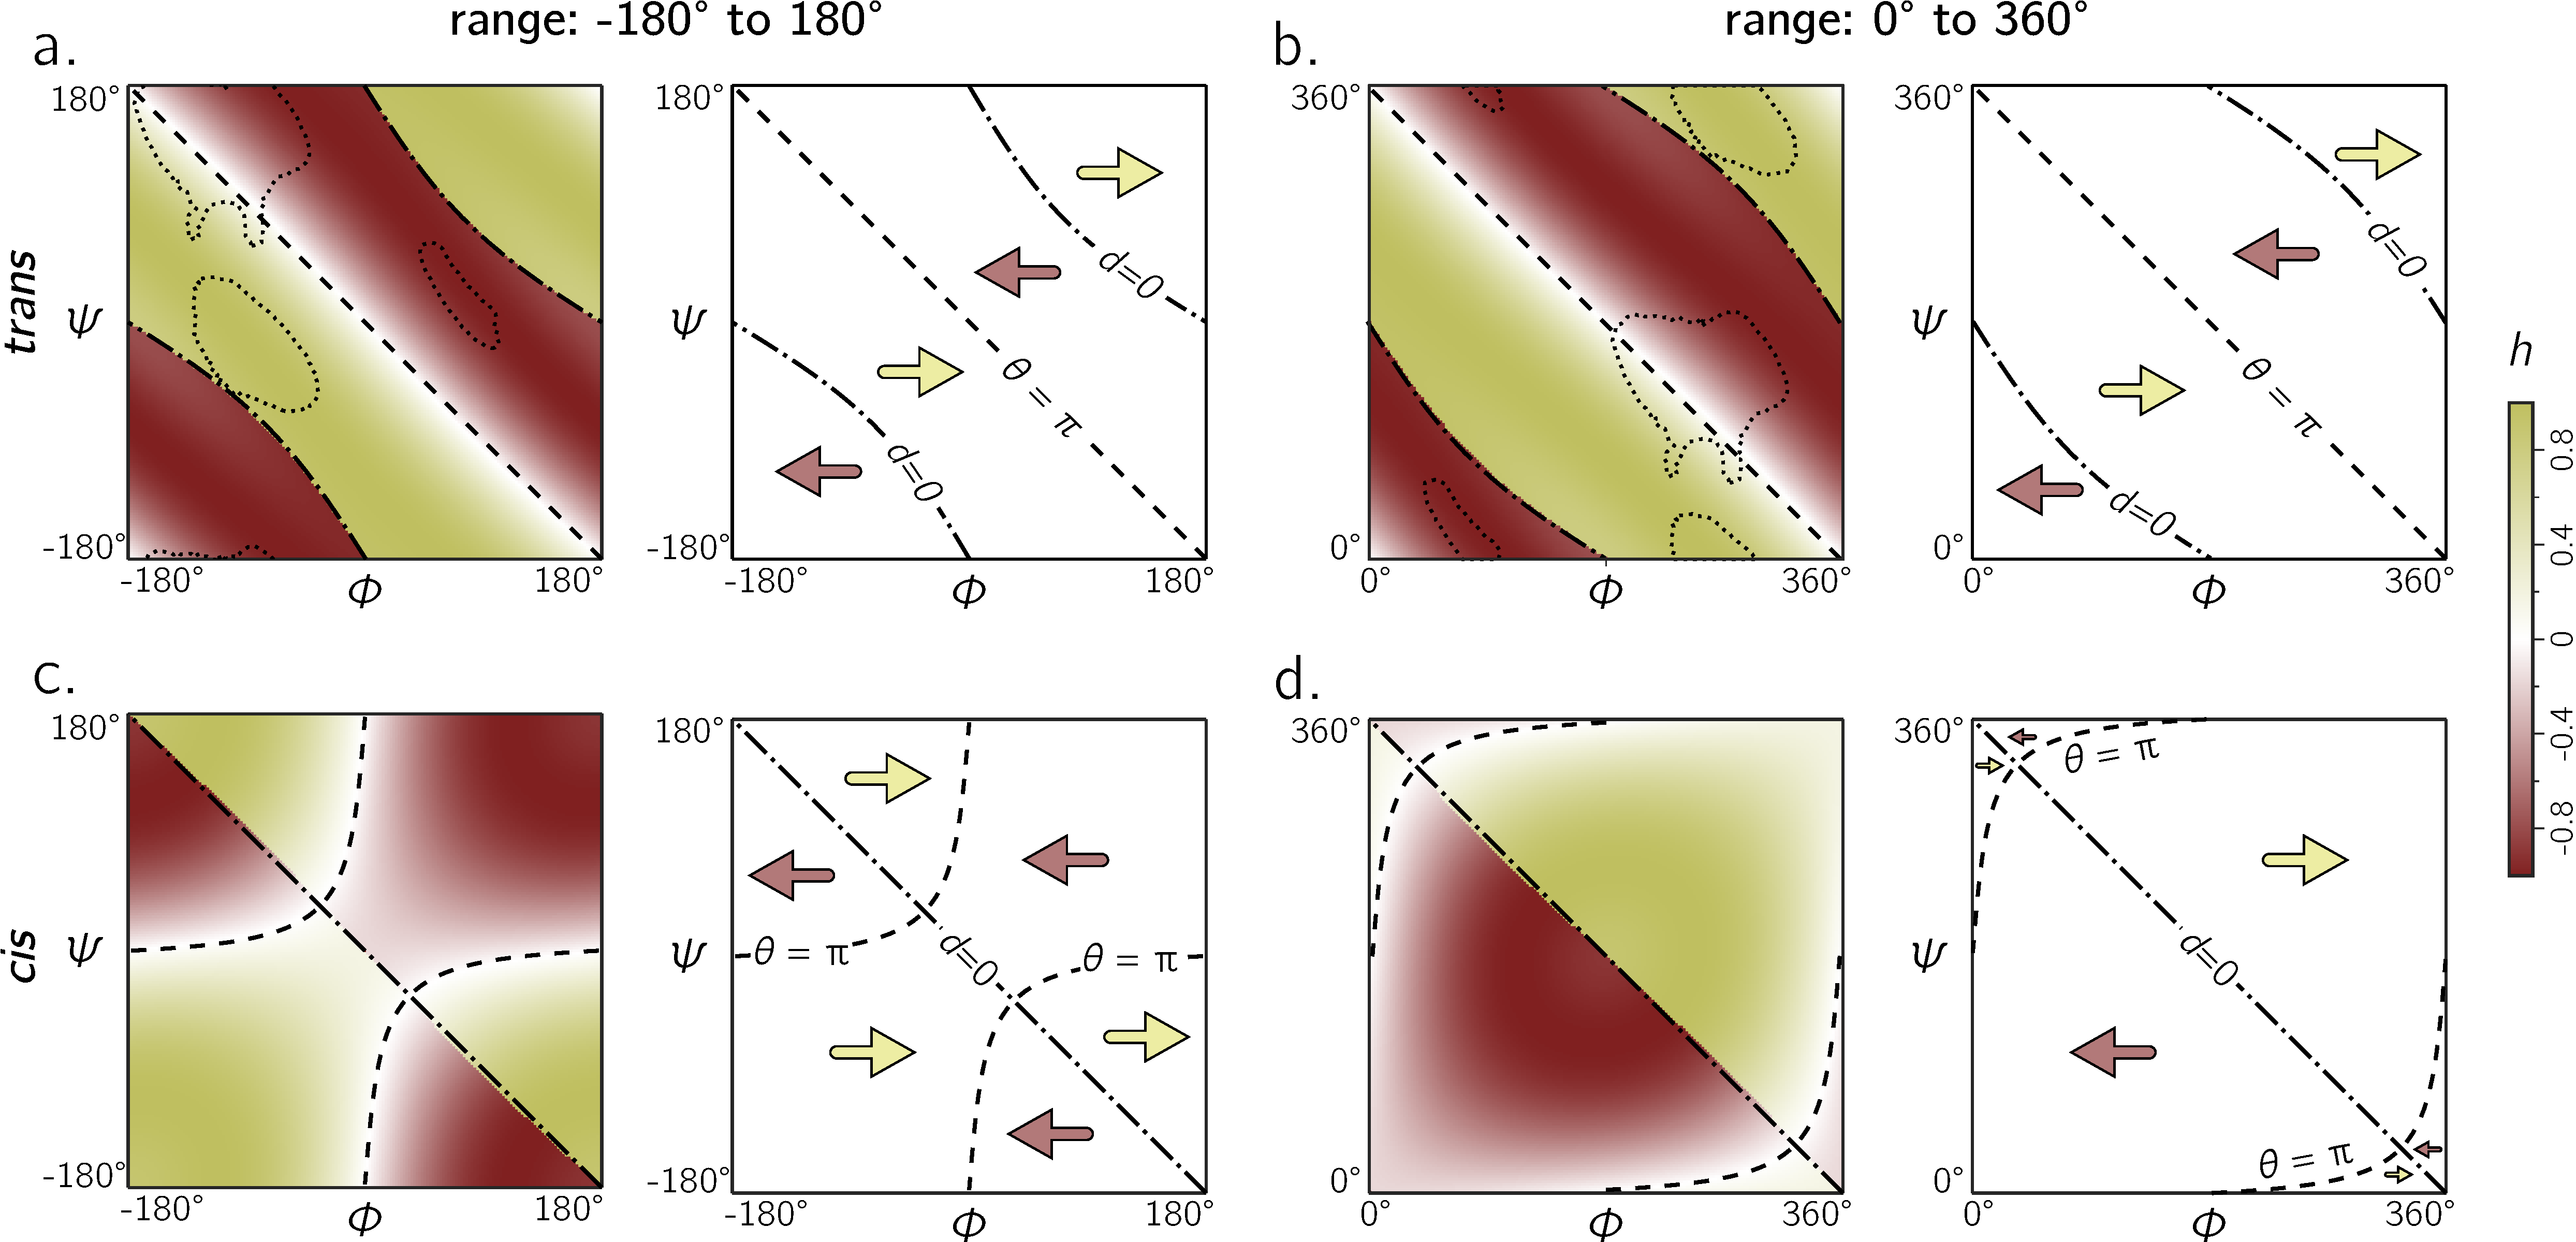
\includegraphics[width=\linewidth]{\figdir/various_chis_skewed.pdf}
\caption{\label{fig:other_chis_skewed} Each panel describes handedness data (right) and boundaries (left). Both frames of references $\left[-\uppi,\ldots,\uppi\right]$ and $\left[0,\ldots,2\uppi\right]$ yield similar trends for $trans$ backbones (a,b); however, for $cis$ backbones, the latter frame of reference (d) appears to more neatly apportion the handedness of the backbone rather than the traditional frame of reference (c). As in \Figs{fig:chi} and~\ref{fig:chi_all}, `\protect\dashedrule' and `\protect\dotdashedrule' respectively correspond to $\theta = \uppi$ and $d=0$.}
\end{figure}

\section*{Conclusions}
\begin{enumerate}%[I]%for capital roman numbers.
\item The handedness of both $cis$ and $trans$ backbones are shown as a function of $\phi$ and $\psi$. 
\item Our na{\"i}ve expectations of handedness is too simple in $trans$ backbones and completely wrong in $cis$ backbones: Each Ramachandran plot contains at least four regions of left- (red) and right-handed (blue) regions (not two), irrespective of the state of the amide dihedral angle. While this was tested for all integer values, the following are some examples ($\phi,\psi \in [-\uppi,\ldots,\uppi]$):\\
~\mbox{}\hfill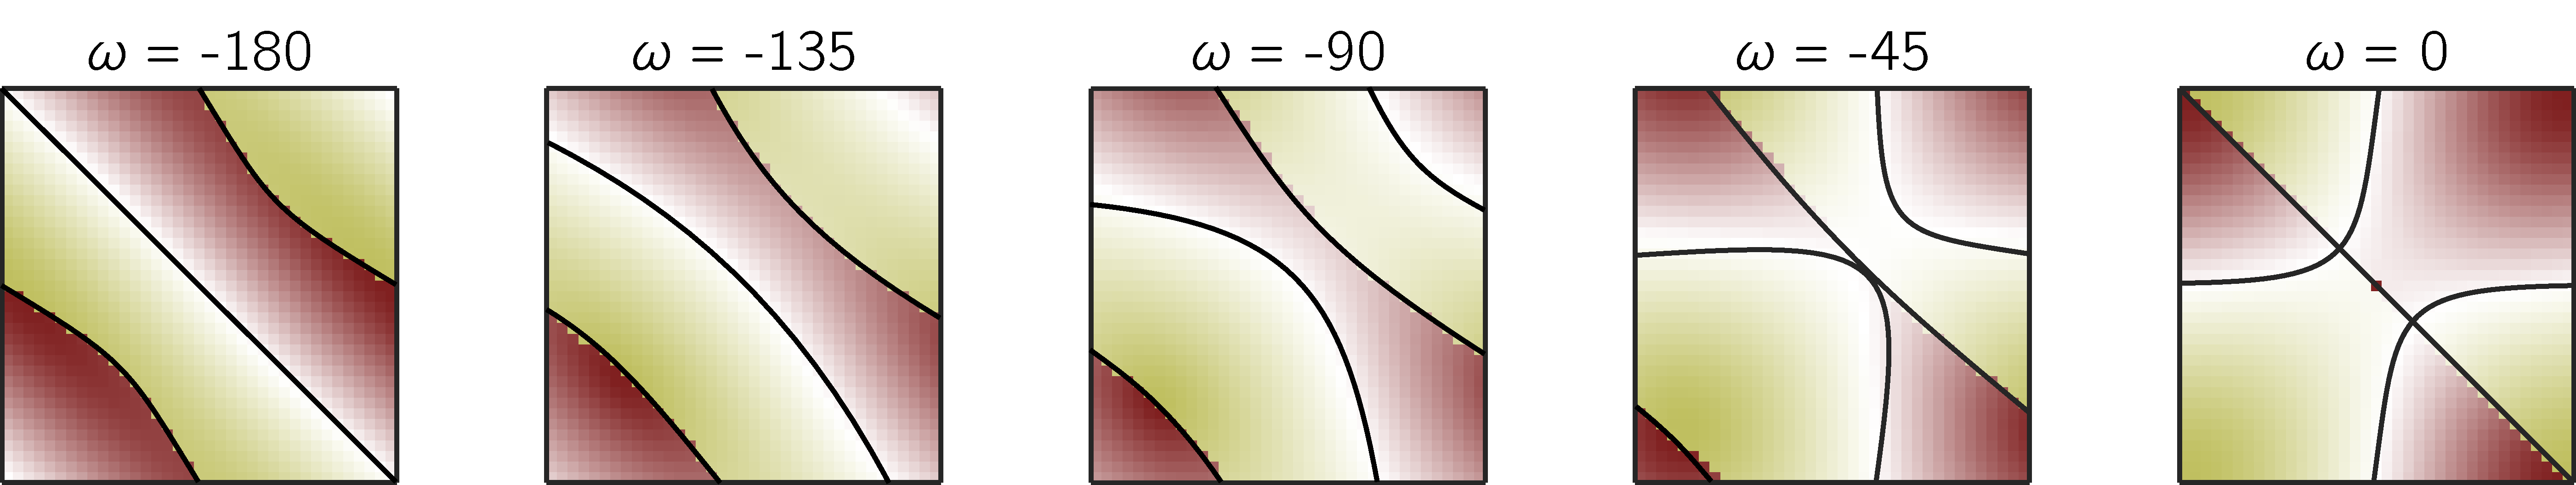
\includegraphics[width=0.7\linewidth]{\figdir/various_omegas.pdf}\hfill\mbox{}~\hfill\mbox{}~
\item Interestingly, the reason for the na{\"i}ve view makes senses when considering only $trans$ peptides: the -ve diagonal (`\protect\dashedrule' in \Figs{fig:chi}a and \ref{fig:chi_all}a) separates $D$ and $L$ twists if we consider only the regions dominantly occupied by structured proteins (`\protect\dottedrule' in \Figs{fig:chi}a and \ref{fig:chi_all}a). 
\item $d=0$ codes for backbones that are flat and optimally extended (for a fixed $theta$).
\item $\theta=\uppi$ codes for backbones that are flat and optimally collapsed or curved (for a fixed $d$).
\item Ramachandran plots have traditionally been shown in the range $[-\uppi,\uppi]$, however, \Fig{fig:other_chis_skewed} indicates that the alternative range -- $[0,2\uppi]$ -- may be more meaningful when considering basic structural properties, especially when considering the $cis$ backbone.
\end{enumerate}

\section*{Acknowledgments}

RVM was supported by the Defense Threat Reduction Agency under contract no. IACRO-B0845281. RVM thanks Alana Canfield Mannige for her input. This work was done at the Molecular Foundry at Lawrence Berkeley National Laboratory (LBNL), supported by the Office of Science, Office of Basic Energy Sciences, of the U.S. Department of Energy under Contract No. DE-AC02-05CH11231.

\bibliography{all}

\end{document}

\section{A new Ramachandran number}

Historically, the range of $\phi$ and $\psi$ within the Ramachandran plot has been $[-\uppi,1802^\circ]$ \citep{Berg2006,Alberts2002,Laskowski1993,Laskowski2003}. 

We divide the plot into a square grid of $(2\uppi \sigma)^2$ sites, where $\sigma$ is a scaling factor that is measured in reciprocal degrees. We shall show that it is straightforward to make $\sigma$ large enough that the error incurred upon converting angles from structures in the protein databank to Ramachandran numbers and back again is less than the characteristic error associated with the coordinates of structures in that database.

Given a choice of grid resolution $\sigma$, we define the integer-valued Ramachandran number for the new frame of reference\cite{MannigeKunduWhitelam2016}:
\beq
\label{ramachandran2}
R_\mathbb{Z}(\phi,\psi)  \equiv \round{\phi'} + \lambda' \round{\psi'},
\eeq
in which the coordinates
\beq
\phi' = (\phi - \psi + \lambda)\sigma/\sqrt{2}
\eeq
\beq
\psi' = (\phi + \psi)\sigma/\sqrt{2}
\eeq 
correspond to a clockwise rotation by 45$^\circ$, a shift, and a rescaling of the original coordinates $\phi$ and $\psi$ (\cite{MannigeKunduWhitelam2016}), and the parameter
And
\beq
\lambda' = \round{\sqrt{2} \lambda \sigma}
\eeq
In these relations the symbol $\round{x}$ means the integer closest to the real number $x$, i.e. $\round{2.49} = 2$ and $\round{2.51} =3$. Combined, the integer-valued Ramachandran number is:
\beq
\label{ramachandran3}
R_\mathbb{Z}(\phi,\psi) \equiv \round{(\phi - \psi + \lambda)\sigma/\sqrt{2}} + \round{\sqrt{2} \lambda\sigma} \round{(\phi+\psi)\sigma/\sqrt{2}}.
\eeq

The integer-valued Ramachandran number runs between $R_{\mathbb{Z},\rm min} = R_{\mathbb{Z}}(-180,-180) = \n{\round{\lambda\sigma/\sqrt{2}}}$ and $R_{\mathbb{Z},\rm max} = R_{\mathbb{Z}}(180,180) = \n{R_{\mathbb{Z},\rm min} + \round{\sqrt{2}\lambda\sigma}^2}$. \n{The range of these values are dependent on $\sigma$, which makes $R_{\mathbb{Z}}$ a difficult value to intuitively grasp. Therefore,} for ease of plotting, we define the real-valued, normalized, Ramachandran number
\beq
\label{ramachandran}
{\mathcal{R}}(\phi,\psi) \equiv  \frac{R_\mathbb{Z}(\phi,\psi)-R_{\mathbb{Z},\rm min}}{R_{\mathbb{Z},\rm max}-R_{\mathbb{Z},\rm min}},
\eeq
which is a value that is practically invariant of $\sigma$. \n{Given that $\phi,\psi \in [-\lambda/2,\lambda/2)$ or $[-180,180)$, the ranges of $R_{\mathbb{Z}}$ and $\mathcal{R}$ are respectively $[R_{\mathbb{Z},\rm min},R_{\mathbb{Z},\rm max})$ and $[0,1)$.} %while $R_{\mathbb{Z},\rm max}$ serves to normalize $\mathcal{R}$, $R_{\mathbb{Z},\rm max} = R_{\mathbb{Z}}(180,180)$ will never be occupied in practice.


\begin{align}
\cos\left(\frac{\theta}{2}\right) =& 0.61434193354 \times\cos\left(\frac{\phi+\psi+\omega}{2}\right) 
                                    -0.20914888365 \times\cos\left(\frac{\phi+\psi-\omega}{2}\right) \nonumber \\
                                   &-0.25772755386 \times\cos\left(\frac{\phi-\psi+\omega}{2}\right)
                                    -0.23549054935 \times\cos\left(\frac{\phi-\psi-\omega}{2}\right)
                                  \label{eqn:theta}
\end{align}
\begin{align} 
d \sin\left(\frac{\theta}{2}\right) = & 2.65395715289 \times\sin\left(\frac{\phi+\psi+\omega}{2}\right)
                                       -0.34467736025 \times\sin\left(\frac{\phi+\psi-\omega}{2}\right)\nonumber \\
                                      &-0.3273139934  \times\sin\left(\frac{\phi-\psi+\omega}{2}\right)
                                       +0.33015775018 \times\sin\left(\frac{\phi-\psi-\omega}{2}\right)
                                    \label{eqn:d}
\end{align}


When $\omega=\uppi$,
\begin{align}
\label{eqn:theta_trans}
\cos\left(\frac{\theta}{2}\right) =&-0.82349081719 \times\sin\left(\frac{\phi+\psi}{2}\right) 
                                    +0.02223700451 \times\sin\left(\frac{\phi-\psi}{2}\right) \\
\label{eqn:d_trans}
d \sin\left(\frac{\theta}{2}\right) =& 2.99863451314 \times\cos\left(\frac{\phi+\psi}{2}\right)
                                      -0.65747174358 \times\cos\left(\frac{\phi-\psi}{2}\right)
\end{align}

When $\omega=0$,
\begin{align}
\label{eqn:theta_cis}
\cos\left(\frac{\theta}{2}\right) =& 0.40519304989 \times\cos\left(\frac{\phi+\psi}{2}\right)
                                    -0.49321810321 \times\cos\left(\frac{\phi-\psi}{2}\right) \\
\label{eqn:theta_d}
d \sin\left(\frac{\theta}{2}\right) = & 2.30927979264 \times\sin\left(\frac{\phi+\psi}{2}\right)
                                       +0.00284375678 \times\sin\left(\frac{\phi-\psi}{2}\right)
\end{align}


%\begin{figure}[h!]
%\centering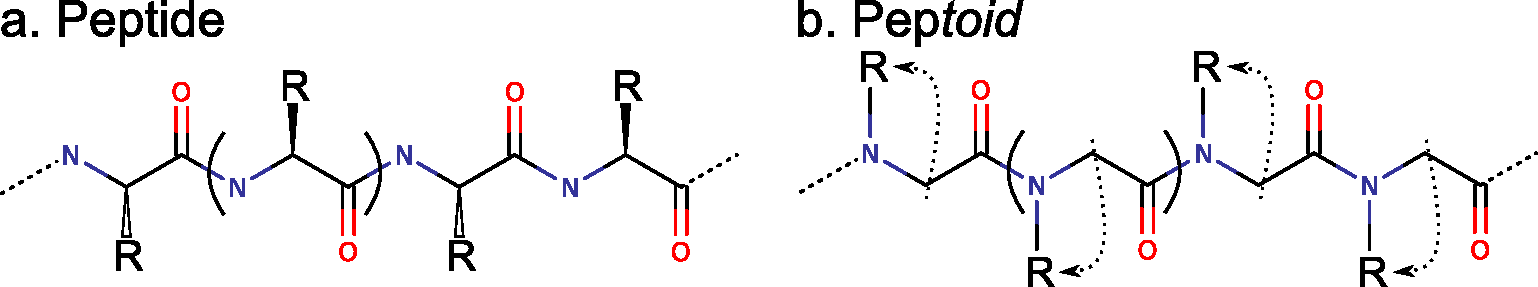
\includegraphics[width=0.9\textwidth]{\figdir/Figure_si_S1b.pdf}
%\caption{{\bf Peptoids and peptides are distinguished by the position of their sidechain (R) groups.} They therefore behave differently. For example, the peptoid backbone is more flexible than the protein one, and peptoid backbones lack canonical hydrogen bond donors, which are crucial to the formation of traditional secondary structures in proteins such as $\upalpha$-helices $\upbeta$-sheet \citep{Berg2006}.\label{FigSIpeptoid}}
%\end{figure}

Backbones of natural amino acids with `L' chirality dominantly occupy the ``left side'' of the plot ($\phi<0$; \Fig{fig_altr}a, top), a consequence of the chirality of the backbone $\upalpha$-carbon \citep{Berg2006,Cintas2002} and steric hindrance between the backbone carbonyl and sidechain atoms (\cite{Branden1999}). Interestingly, switching the C$_\upalpha$'s chirality for every residue results in structures that exist on the ``other side'' of the plot, which a majority of its density at $\phi>0$; (\cite{Zawadzke1993,Hung1998}).

%In addition to a new class of peptide mimcs requiring a reassesment of the historically `less-traveled' regions of the Ramachandran plot: DISORDER.  Additionally, a number of proteins undergo conformational transitions, without which they may not properly function. Finally, some proteins -- intrinsically disordered proteins -- display massive disorder whose conformations dramatically change over time \citep{Uversky2003, Fink2005, Midic2009, Espinoza-Fonseca2009, Uversky2010, Tompa2011, Sibille2012, Kosol2013, Dunker2013, Geist2013, Mannige2014, Baruah2015}.

%Many of the useful/distinguishing structural properties of peptoids emerge from the primary feature that distinguishes peptoids from peptides: peptoid sidechains are attached to backbone nitrogen atoms rather than backbone $\upalpha$-carbon atoms (\Fig{FigSIpeptoid}). Interestingly, this change in the sidechain's position drastically alters the structural and dynamical properties of the peptoid backbone (e.g., protein secondary structure facilitating hydrogen bond donors are missing in peptoids\cite{Berg2006,Matsuurua2014}). These unique properties allow for peptoids of specific sequences to form a wide range of stable structures\cite{Paul2011,Butterfoss2012,Yoo2008,Shah2008,Laursen2013,Butterfoss2009,Nam2010}.
%Particularly relevant from a design perspective, some peptoids have been shown to display structures -- self-healing membrane-like peptoids\cite{Haibao2016} and peptoid nanosheets\cite{Nam2010,Sanii2011,Kudirka2011,Mannige2015} -- that are nanoscale in some dimensions and mescoscopic in other dimensions. Such atomistically intricate yet mesoscopic assemblies are unseen in natural proteins, and serve as proof-of-concepts for the further search for novel peptoid assemblies. However, unlike evolution's considerable sampling capabilities, the discovery of such novel peptoid structures and assemblies are limited to the speed at which chemists are able to design and produce such molecules. This limitation raises the utility of the high-throughput exploration of peptoid chemistry and structure with the help of computational simulation.
